% Let \(X\) be \textcolor{red}{a connected graph with at least one arrow}  \textcolor{blue}{a graph with no isolated nodes}, and let \(\rho = (l, r)\) be a rewriting rule that has more morphisms from \(X\) to the input graph than to the output graph. Consider the commutative diagram depicted below, where the squares \(\square KLGC\), \(\square KCHR\), and \(\square KCH'R_X\) are pushout squares:

% \begin{figure}[htbp] 
%     \center
%     \begin{tikzpicture}
%         \node (k) at (0,1) {K};
%         \node (l) at (-2,1) {L};
%         \node (r) at (2,1) {R};
%         \node (c) at (0,-2) {C};
%         \node (g) at (-2,-2) {G};
%         \node (h) at (2,-2) {H};
%         % \node (t) at (0,-4) {T};
%         \node (rb) at (1.5,-0.5) {$R_X$};
%         \node (h') at (1.5,-1.5) {$H'$};
%         % \draw[>->]  (h') -- (t) node [midway] {!};
%         \draw[>->]  (rb) -- (h') node [midway,above] {};
%         \draw[>->]  (c) -- (h') node [midway,above] {};
%         \draw[<-<]  (l) -- (k) node [midway,above] {$l$};
%         \draw[>->]  (k) -- (r) node [midway,above] {$r$};
%         \draw[>->] (c) -- (g) node [midway, below] {};
%         \draw[>->] (c) -- (h) node [midway,below] {};
%         \draw[>->] (l) -- (g) node[midway, left] {};
%         \draw[>->] (r) -- (h) node[midway, right] {};
%         \draw[>->] (k) -- (c) node[midway, left] {};
%         \draw[>->] (rb) to (r);
%         \draw[->] (rb) to (l);
%         \draw[<-<] (rb) to (k);
%         % \draw [->]  (rb) to
%         % (t) ;
%         % \draw [->]  (l) to [out=-140, in=180] (t) ;
%         % \draw [->]  (r) to [out=-50, in=0] (t) ;
%         % \draw [->] (c) to (t);
%     \end{tikzpicture}
%     \caption{}
%     \label{fig:lem:w_u_l_not_geq_r_not}
% \end{figure}

% % Let $t_X$, $t_G, t_{H'}$ and $t_H$ be the unique graph homomorphisms from $X$, $G, H'$ and $H$ to $T_\Sigma^X$, defined in Definition~\ref{def:t_sigm_x}.
% Let \(t_X\), \(t_G\), \(t_{H'}\), and \(t_H\) be the unique graph homomorphisms from \(X\), \(G\), \(H'\), and \(H\) to \(T_\Sigma^X\), as defined in Definition~\ref{def:t_sigm_x}. We define 


% \begin{flalign*}
%     \Psi_{G,\lnot L,\lnot C} \overset{\operatorname*{def}}{=} \{ 
%     \iota : X \to G \ |\ \nexists \zeta: X \to L.~\iota &= \zeta \star h_{LG} ~\land\\
%                         \nexists \eta: X \to C.~\iota &= \eta \star h_{CG} ~
%                 %         \land\\
%                 %  t_X &= \iota \star t_G 
%     ~\}
%     \\
%    \operatorname{Hom}(X, H', \lnot h_{R_XH'}, \lnot h_{CH'}) \overset{\operatorname*{def}}{=} \{ 
%     \iota: X \to H' \ |\ \nexists \zeta:X \to R_X.~\iota &= \zeta \star h_{R_XH'} \land              \\ \nexists \eta: X \to C.~\iota &= \eta \star h_{CH'}
%     %\\  t_X &= \iota \star t_{R_X}
%         ~\}
%     \\
%     \operatorname{Hom}(X, H, \lnot m'', \lnot r') \overset{\operatorname*{def}}{=} \{ 
%         \iota:X \to H \ |\ \nexists \zeta : X \to R.~\iota &= \zeta \star h_{RH} \land\\ \nexists \eta:X \to C.~\iota &= \eta \star h_{CH} 
%        % \land   \\ t_X &= \iota \star t_H
%             ~\}
% \end{flalign*}

\noindent\begin*{\textbf{\autoref{lem:w_u_l_not_geq_r_not}}}
    Let $X$ be a graph with no isolated nodes. Let  $L \overset{l}{\leftarrow} K \overset{r}{\rightarrow} R$ be a graph rewriting rule with $l$ arrow-injective and $r$ node-injective.
    Suppose that $\rho$ does not increase the number of morphisms from \(X\). Consider the commutative diagram $\delta$ of the form: 
\begin{center}
    \resizebox{0.4\textwidth}{!}{
            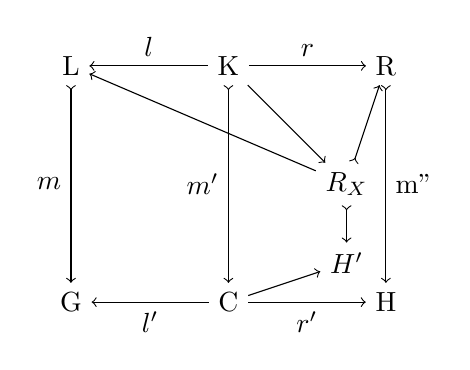
\begin{tikzpicture}
        \node (k) at (0,1) {K};
        \node (l) at (-2,1) {L};
        \node (r) at (2,1) {R};
        \node (c) at (0,-2) {C};
        \node (g) at (-2,-2) {G};
        \node (h) at (2,-2) {H};
        \node (rb) at (1.5,-0.5) {$R_X$};
        \node (h') at (1.5,-1.5) {$H'$};
        \draw[>->]  (rb) -- (h') node [midway,above] {};
        \draw[->]  (c) -- (h') node [midway,above] {};
        \draw[<-]  (l) -- (k) node [midway,above] {\(l\)};
        \draw[->]  (k) -- (r) node [midway,above] {\(r\)};
        \draw[->] (c) -- (g) node [midway, below] {$l'$};
        \draw[->] (c) -- (h) node [midway,below] {$r'$};
        \draw[>->] (l) -- (g) node[midway, left] {$m$};
        \draw[>->] (r) -- (h) node[midway, right] {m''};
        \draw[>->] (k) -- (c) node[midway, left] {$m'$};
        \draw[>->] (rb) to (r);
        \draw[->] (rb) to (l);
        \draw[<-] (rb) to (k);
    \end{tikzpicture}
    }
\end{center}
where $\square KLGC,\square KCHR$ and $\square KCH'R_X$ are pushout squares. We have
\[
    |\operatorname{Hom}(X, H, \lnot m'', \lnot r')| \leq |\operatorname{Hom}(X, H', \lnot h_{R_XH'}, \lnot h_{CH'})| \leq |\operatorname{Hom}(X, G, \lnot m, \lnot l')|
    \]
% where
%     \begin{flalign*}
%         \operatorname{Hom}(X, H, \lnot m'', \lnot r') \overset{\operatorname*{def}}{=} \{ 
%             \iota:X \to H \ |\ \nexists \zeta : X \to R.~\iota &= \zeta \star h_{RH} \land\\ \nexists \eta:X \to C.~\iota &= \eta \star h_{CH} 
%         % \land   \\ t_X &= \iota \star t_H
%                 ~\}
%                 \\
%         \Psi_{G, \lnot L,\lnot C} \overset{\operatorname*{def}}{=} \{ 
%         \iota : X \to G \ |\ \nexists \zeta: X \to L.~\iota &= \zeta \star h_{LG} ~\land\\
%                             \nexists \eta: X \to C.~\iota &= \eta \star h_{CG} ~
%                     %         \land\\
%                     %  t_X &= \iota \star t_G 
%         ~\}
%         \\
%     \operatorname{Hom}(X, H, \lnot m'', \lnot r') \overset{\operatorname*{def}}{=} \{ 
%         \iota: X \to H' \ |\ \nexists \zeta:X \to R_X.~\iota &= \zeta \star h_{R_XH'} \land              \\ \nexists \eta: X \to C.~\iota &= \eta \star h_{CH'}
%         %\\  t_X &= \iota \star t_{R_X}
%             ~\}        
%     \end{flalign*}
 \end*{}
 \begin{proof}
    \label{proof_w_u_l_not_geq_r_not}
%    By Definition~\ref{def:weight_excluding},
    % \begin{flalign*}
    %     w_{\mathcal{T}_\Sigma^X}(t_G - \{h_{LG}, h_{CG}\}) &= |\operatorname{Hom}(X, H', \lnot h_{R_XH'}, \lnot h_{CH'})| \\
    %     w_{\mathcal{T}_\Sigma^X}(t_{H'} - \{h_{R_XH'}, h_{CH'}\}) &= |\operatorname{Hom}(X, H', \lnot h_{R_XH'}, \lnot h_{CH'})| \\
    %     w_{\mathcal{T}_\Sigma^X}(t_H - \{h_{RH}, h_{CH}\}) &= |\operatorname{Hom}(X, H, \lnot m'', \lnot r')|
    % \end{flalign*}
    % Therefore, it is equivalent to prove 
    % \[
    % |\operatorname{Hom}(X, H, \lnot m'', \lnot r')| \leq |\operatorname{Hom}(X, H', \lnot h_{R_XH'}, \lnot h_{CH'})| \leq |\operatorname{Hom}(X, H', \lnot h_{R_XH'}, \lnot h_{CH'})|
    % \]

    % By~\autoref{lem:2_exist} and~\autoref{lem:2_distinct}, there exists an injective function $\mathbb{G} : \homset{X}{H} \to \homset{X}{H'}$. Therefore, $\mathbb{G}(\operatorname{Hom}(X, H, \lnot m'', \lnot r')) \subseteq \operatorname{Hom}(X, H', \lnot h_{R_XH'}, \lnot h_{CH'})$. Thus, $|\operatorname{Hom}(X, H, \lnot m'', \lnot r')| \leq |\operatorname{Hom}(X, H', \lnot h_{R_XH'}, \lnot h_{CH'})|$.

    % By~\autoref{lem:1_ex} and~\autoref{lem:1_dist}, there exists an injective function $\mathbb{F} : \homset{X}{H'} \to \homset{X}{G}$. Therefore, $\mathbb{F}(\operatorname{Hom}(X, H', \lnot h_{R_XH'}, \lnot h_{CH'})) \subseteq \operatorname{Hom}(X, H', \lnot h_{R_XH'}, \lnot h_{CH'})$. Hence, $|\operatorname{Hom}(X, H', \lnot h_{R_XH'}, \lnot h_{CH'})| \leq |\operatorname{Hom}(X, H', \lnot h_{R_XH'}, \lnot h_{CH'})|$.

    By~\autoref{lem:1_ex} and~\autoref{lem:1_dist}, there exists an injective function $\mathbb{F} : \operatorname{Hom}(X, H', \lnot h_{R_XH'}, \lnot h_{CH'}) \to \operatorname{Hom}(X, G, \lnot m, \lnot l')$. Hence, $|\operatorname{Hom}(X, H', \lnot h_{R_XH'}, \lnot h_{CH'})| \leq |\operatorname{Hom}(X, H', \lnot h_{R_XH'}, \lnot h_{CH'})|$.
   
    By~\autoref{lem:2_exist} and~\autoref{lem:2_distinct}, there exists an injective function $\mathbb{G} : \operatorname{Hom}(X, H, \lnot m'', \lnot r') \to \operatorname{Hom}(X, H', \lnot h_{R_XH'}, \lnot h_{CH'})$. Thus, $|\operatorname{Hom}(X, H, \lnot m'', \lnot r')| \leq |\operatorname{Hom}(X, H', \lnot h_{R_XH'}, \lnot h_{CH'})|$.

\end{proof}  



% \begin{lemma}
%     \label{lem:b_notin_imhab_no_c_with_sameimg}

%     Consider the pushout square \( \Delta \) depicted below:

%     \begin{center}{\normalfont
%         \begin{tikzpicture}[node distance=12mm]
%             \node (A) {$A$};
%             \node (B) [right of=A] {$B$};
%             \node (C) [below of=A] {$C$};
%             \node (D) [right of=C] {$D$};
%             \draw [>->] (A) to (B);
%             \draw [>->] (A) to (C);
%             \draw [>->] (B) to (D);
%             \draw [>->] (C) to (D);
%         \end{tikzpicture}
%     }\end{center}

%     If $b \in B \setminus \operatorname{Im}(h_{AB})$, then there is no $c \in C$ such that $h_{BD}(b) = h_{CD}(c)$.
% \end{lemma}


% \begin{lemma}
%     \label{lem:x_notin_im_h_ab}
%     Consider the commutative diagram depicted below:
%     \begin{center}
%         \begin{tikzpicture}[node distance=2cm, auto]
%           \node (A) {$A$}; 
%           \node [right of=A] (B) {$B$}; 
%           \node [below of=A] (C) {$C$}; 
%           \node [below of=B] (D) {$D$}; 
          
%           \draw[>->] (A) -- node {$\alpha$} (B);
%           \draw[>->] (A) -- node [swap] {$\beta$} (C);
%           \draw[>->] (B) -- node {$\beta'$} (D); 
%           \draw[>->] (C) -- node [swap] {$\alpha'$} (D);
%         \end{tikzpicture}
%     \end{center}

%     \begin{itemize}
%         \item \label{lem:b_c_same_img_exist_a:1} For all \(b \in B \setminus \operatorname{Im}(\alpha)\) and \(c \in C\), we have \(\beta'(b) \neq \alpha'(c)\).
%     \end{itemize}
    
% \end{lemma}

% \begin{proof}
%     Suppose, by contradiction, that there exist \(b \in B \setminus \operatorname{Im}(\alpha)\) and \(c \in C\) such that \(\beta'(b) = \alpha'(c)\). By~\autoref{lem:b_c_same_img_exist_a}, there exists \(a \in A\) such that \(\alpha(a) = b\). This contradicts the assumption that \(b \notin \operatorname{Im}(\alpha)\) since \(\alpha(a) = b\) implies \(b \in \operatorname{Im}(\alpha)\).  
% \end{proof}


% \begin{lemma}
%     \label{lem:dpo_dpo_unique_homo}

%     Consider the commutative diagram depicted below:
    
%     \begin{center}
%     \resizebox{3cm}{!}{
%         \begin{tikzpicture}
%             \node (k') {K'};
%             \node (c') [below=of k'] {C'};
%             \node (c) [below=of c'] {C};
%             \node (x) [right=of c'] {X};
%             \node (r') [right=of k'] {R'};
%             \node (rb) [right=of r'] {$R_X$};
%             \node (h') [right=26mm of c] {$H'$};
%             \node () [at=($(k')!.5!(x)$)] {$PO$};
%             \draw[->]  (rb) -- (h')  {};
%             \draw[->]  (c) -- (h'){};
%             \draw [->] (x) -- (h');
%             \draw [->] (c') -- (x);
%             \draw [->] (r') -- (x);
%             \draw [->] (c') -- (c);
%             \draw [->] (r') -- (rb);
%             \draw [->] (k') -- (r');
%             \draw [->] (k') -- (c');
%     \end{tikzpicture}
%     }
% \end{center}

%     The homomorphism $h_{XH'}$ is the unique morphism such that $h_{C'X} \star h_{XH'} = h_{C'C} \star h_{CH'}$ and $h_{R'X} \star h_{XH'} = h_{R'R_X} \star h_{R_XH'}$.
% \end{lemma}
% \begin{proof}
%     We have $h_{C'C} \star h_{CH'} = h_{C'X} \star h_{XH'}$ and $h_{R'R_X} \star h_{R_XH'} = h_{R'X} \star h_{XH'}$ from the commutativity of $\square C'CH'X$ and $\square R'XH'R_X$. The uniqueness follows from the universal mapping property of the pushout $\square K'C'XR'$ and
%     \begin{flalign*}
%         h_{K'C'} \star h_{C'C} \star h_{CH'} & = h_{K'C'} \star h_{C'X} \star h_{XH'} & \text{by commutativity of $\square C'CH'X$}\\
%         & = h_{K'R'} \star h_{R'X} \star h_{XH'} & \text{by commutativity of $\square K'C'XR'$} \\
%         & = h_{K'R'} \star h_{R'R_X} \star h_{R_XH'} & \text{by commutativity of $\square R'XH'R_X$}
%     \end{flalign*}
%     \qed
% \end{proof}


% \begin{lemma}
%     \label{lem:dpo_dpo_unique_homo}

%     Consider the commutative diagram depicted below:
    
%     \begin{tikzpicture}
%         \def\scl{2}
%         \node (c) at ($\scl*(0,-1.5)$) {C};
%         \node (rb) at ($\scl*(1.5,-0.5)$) {$R_X$};
%         \node (h') at ($\scl*(1.5,-2)$) {$H'$};
%         \draw[>->]  (rb) -- (h') node [midway,above] {};
%         \draw[>->]  (c) -- (h') node [midway,above] {};
%        \node (k') at ($\scl*(0.3,-0.6)$) {K'};
%         \node (r') at ($\scl*(0.8,-0.6)$) {R'};
%         \node (c') at ($\scl*(0.3,-1)$) {C'};
%         \node (x) at ($\scl*(.8,-1)$) {X};
%         \node () at ($\scl*(0.55,-1.4)$) {=};
%         \node () at ($\scl*(1.3,-1)$) {=};
%          \node () at ($\scl*(0.55,-0.8)$) {$PO$};
%         \draw [->] (x) -- (h');
%         \draw [>->] (c') -- (x);
%         \draw [>->] (r') -- (x);
%         \draw [->] (c') -- (c);
%         \draw [->] (r') -- (rb);
%        \draw [>->] (k') -- (r');
%         \draw [>->] (k') -- (c');
%     \end{tikzpicture}

%  Homomorphism $h_{XH'}$ is the unique morphism such that $h_{C'X} \star h_{XH'} = h_{C'C} \star h_{CH'}$ and $h_{R'X} \star h_{XH'} = h_{R'R_X} \star h_{R_XH'}$ 
% \end{lemma}
% \begin{proof}
%     we have $ h_{K'C'} \star h_{C'C} \star h_{CH'} = h_{K'R'} \star h_{R'R_X} \star h_{R_XH'} $ by~\autoref{lem:dpo_dpo_unique_homo}. By the universal mapping property of the pushout $\square K'C'XR'$, we conclude.
%     \qed
% \end{proof}

\begin{lemma} 
    \label{lem:nincl}
    Consider the commutative diagram depicted below:

    \begin{center}
    \resizebox{3cm}{!}{
        \begin{tikzpicture}
        \def\scl{2}
        \node (k) at ($\scl*(0,0)$) {K};
        \node (c) at ($\scl*(0,-1.5)$) {C};
        \node (rb) at ($\scl*(1.5,-0.5)$) {$R_X$};
        
        \node (h') at ($\scl*(1.5,-2)$) {$H'$};
        \draw[>->]  (rb) -- (h') node [midway,above] {};
        \draw[->]  (c) -- (h') node [midway,above] {};
        \draw[>->] (k) -- (c) node[midway, left] {};
        \draw[<-] (rb) to (k);
        \node (k') at ($\scl*(0.3,-0.6)$) {K'};
        \node (r') at ($\scl*(0.8,-0.6)$) {R'};
        \node (c') at ($\scl*(0.3,-1)$) {C'};
        \node (x) at ($\scl*(.8,-1)$) {X};
        \node () at ($\scl*(0.55,-0.8)$) {$PO$};
        % \node () at ($\scl*(0.55,-1.4)$) {=};
        % \node () at ($\scl*(1.3,-1)$) {=};
        \draw [->] (x) -- (h');
        \draw [->] (c') -- (x);
        \draw [>->] (r') -- (x);
        \draw [->] (k') -- (r');
        \draw [>->] (k') -- (c');
        \draw [->] (c') -- (c);
        \draw [->] (r') -- (rb);
    \end{tikzpicture}
    }
    \end{center}

    If $h_{XH'} \in \operatorname{Hom}(X, H', \lnot h_{R_XH'}, \lnot h_{CH'})$, then we have $\operatorname{Im}(h_{C'C})  \not \subseteq \operatorname{Im}(h_{KC})$ and $\operatorname{Im}(h_{R'R_X}) \not \subseteq  \operatorname{Im}(h_{KR_X}) $
\end{lemma}
\begin{proof}
   
    Suppose \(h_{XH'} \in \operatorname{Hom}(X, H', \lnot h_{R_XH'}, \lnot h_{CH'})\). By symmetry, it suffices to prove that \(\operatorname{Im}(h_{C'C}) \not\subseteq \operatorname{Im}(h_{KC})\). 
    
    Suppose, by contradiction, that 
        \begin{flalign*}
            \operatorname{Im}(h_{C'C}) \subseteq \operatorname{Im}(h_{KC}) \tag{hyp1}\label{lem:nincl:hyp1}
        \end{flalign*} We will show that this assumption leads to the existence of a morphism \(\zeta : X \to R_X\) such that \(h_{XH'} = \zeta \star h_{R_XH'}\), which contradicts the premise \(h_{XH'} \in \operatorname{Hom}(X, H', \lnot h_{R_XH'}, \lnot h_{CH'})\), where no such morphism \(\zeta\) should exist.

   Given the monicity of \(h_{KC}\) and \eqref{lem:nincl:hyp1}, we can define a graph homomorphism \(h_{C'K}\) such that for any \(c' \in C'\), we have \(h_{C'K}(c') \overset{\operatorname{def}}{=} k \in K\), where \(k\) is the unique element in \(K\) satisfying \(h_{KC}(k) = h_{C'C}(c')\). We then have:
\begin{flalign*}
    h_{C'K} \star h_{KC} = h_{C'C} \tag{0} \label{eq:h_cpk_star_h_kc_eq_h_cpc}
\end{flalign*}

The following equation follows:
\begin{flalign*}
    (h_{K'C'} \star h_{C'K} \star h_{KR_X}) \star h_{R_XH'} = (h_{K'R'} \star h_{R'R_X}) \star h_{R_XH'} \tag{1} \label{hrxhpm}
\end{flalign*}
because:
\begin{flalign*}
    & (h_{K'C'} \star h_{C'K} \star h_{KR_X}) \star h_{R_XH'} & \\
    = & h_{K'C'} \star h_{C'K} \star (h_{KR_X} \star h_{R_XH'}) & \text{by associativity} \\
    =& h_{K'C'} \star h_{C'K} \star (h_{KC} \star h_{CH'}) & \text{by commutativity of $\square KCH'R_X$} \\
    =& h_{K'C'} \star (h_{C'K} \star h_{KC}) \star h_{CH'} & \text{by associativity} \\
    =& h_{K'C'} \star  h_{C'C}  \star h_{CH'} & \text{by \eqref{eq:h_cpk_star_h_kc_eq_h_cpc}} \\
    =& h_{K'R'} \star h_{R'R_X}  \star h_{R_XH'} & \text{by commutativity of $K'C'CH'R_XR'$}\\
    =& (h_{K'R'} \star h_{R'R_X})  \star h_{R_XH'} & \text{by associativity}
\end{flalign*}

By \eqref{hrxhpm} and the monicity of \(h_{R_XH'}\), we deduce:
\begin{flalign*}
    h_{K'C'} \star h_{C'K} \star h_{KR_X} = h_{K'R'} \star h_{R'R_X} \tag{2} \label{hkpc_star_hcpk_star_hkrx}
\end{flalign*}

Thus, the commutative diagram depicted below holds:


    \begin{center}
    \resizebox{4cm}{!}{
        \begin{tikzpicture}
            \node (x) {X};
            \node (k) [below=of x] {K};
            \node (rb) [right=of x] {$R_X$};
            \node (c') [below left=of x] {C'};
            \node (k') [above left=of c'] {K'};
            \node (r') [above left=of x] {R'};
            \node () [at=($(k')!0.5!(x)$)] {$PO$};
            \draw[<-] (rb) to (k);
            % \node (h') at ($\scl*(1.5,-2)$) {$H'$};
            \draw [->] (k') -- (r');
            \draw [>->] (k') -- (c');
            \draw [->] (c') -- (k);
            \draw [->] (r') -- (rb);
            % \draw[>->]  (rb) -- (h') node [midway,above] {};
            % \draw [->] (x) -- (h') node[midway] {!};
            % \draw [->,dashed,red] (x) -- (rb) node[midway] {!};
            \draw [>->] (r') -- (x);
            \draw [->] (c') -- (x);
            % \node () at ($\scl*(2.5,0)$) {=};
        \end{tikzpicture}
    }
    \end{center}
    
    By \eqref{hkpc_star_hcpk_star_hkrx} and the universal mapping property of the pushout $\square K'C'XR'$, there exists a unique morphism $h_{XR_X}$ such that
 
        \begin{flalign*}
            h_{C'X} \star h_{XR_X} &= h_{C'K} \star h_{KR_X} \tag{3} \label{hcpx_star_hxrx}\\
            h_{R'X} \star h_{XR_X} &= h_{R'R_X} \tag{4} \label{hrpx_star_hxrx}
        \end{flalign*}   

    Subsequently, we have 
    \begin{flalign*}
        h_{C'X} \star (h_{XR_X} \star  h_{R_XH'}) &= h_{C'C} \star  h_{CH'} \tag{5} \label{eq5} \\
        h_{R'X} \star (h_{XR_X} \star  h_{R_XH'}) &=  h_{R'R_X} \star  h_{R_XH'} \tag{6} \label{eq6}
    \end{flalign*} because
    \begin{flalign*}
        & h_{C'X} \star (h_{XR_X} \star  h_{R_XH'})  &  \\
        = &( h_{C'X} \star h_{XR_X}) \star  h_{R_XH'}  & \text{by associativity}  \\
        =  & (h_{C'K} \star h_{KR_X}) \star h_{R_XH'}  & \text{by \eqref{hcpx_star_hxrx}}\\
        =  & h_{C'K} \star (h_{KR_X} \star h_{R_XH'})  & \text{by associativity}\\
        =  & h_{C'K} \star (h_{KC} \star  h_{CH'})  & \text{by commutativity of $\square KCH'R_X$}\\
        =  & (h_{C'K} \star h_{KC}) \star  h_{CH'}  & \text{by associativity}\\
        =  & h_{C'C} \star  h_{CH'}  & \text{by \eqref{eq:h_cpk_star_h_kc_eq_h_cpc}}\\
    \end{flalign*}
    and 
    \begin{flalign*}
        & h_{R'X} \star (h_{XR_X} \star  h_{R_XH'})    \\
        = &  (h_{R'X} \star h_{XR_X}) \star  h_{R_XH'} & \text{by associativity}  \\
        =&  h_{R'R_X} \star  h_{R_XH'}  & \text{by \eqref{hrpx_star_hxrx}}  \\
    \end{flalign*}

    Furthermore, by assumption, we have 
    \begin{flalign*}
        h_{C'X} \star h_{XH'} &= h_{C'C} \star  h_{CH'} \tag{7} \label{eq7} \\
        h_{R'X} \star h_{XH'} &=  h_{R'R_X} \star  h_{R_XH'} \tag{8} \label{eq8}
    \end{flalign*}

    By the universal mapping property of the pushout square $\square K'C'XR'$,
    there exists a unique morphism $\iota : X \to H'$ such that 
    \begin{flalign*}
        h_{C'X} \star \iota &= h_{C'C} \star  h_{CH'}   \\
        h_{R'X} \star \iota &=  h_{R'R_X} \star  h_{R_XH'}  
    \end{flalign*}

    Consequently, we confirm $h_{XH'} = h_{XR_X} \star h_{R_XH'}$.
    
    % because under this assumption, there are no morphisms $h_{XR_X}$ satisfying $h_{XH'} = h_{XR_X} \star h_{R_XH'}$. Hence, $h_{C'C}(C') \not \subseteq h_{KC}(K)$ holds.
    \qed 
\end{proof}

\begin{lemma}
    \label{lem:cp_in_mcp_and_rp_in_mrp}
    % Let \(X\) be a connected graph.
     Consider the commutative diagram depicted below, where \(\square KCH'R_X\) is a pushout square:

    \begin{center}
    \resizebox{4cm}{!}{
        \begin{tikzpicture}
        \def\scl{2}
        \node (k) at ($\scl*(0,0)$) {K};
        \node (c) at ($\scl*(0,-1.5)$) {C};
        \node (rb) at ($\scl*(1.5,-0.5)$) {$R_X$};
        
        \node (h') at ($\scl*(1.5,-2)$) {$H'$};
        \draw[>->]  (rb) -- (h') node [midway,above] {};
        \draw[>->]  (c) -- (h') node [midway,above] {};
        \draw[>->] (k) -- (c) node[midway, left] {};
        \draw[<-<] (rb) to (k);
        \node (k') at ($\scl*(0.3,-0.6)$) {K'};
        \node (r') at ($\scl*(0.8,-0.6)$) {R'};
        \node (c') at ($\scl*(0.3,-1)$) {C'};
        \node (x) at ($\scl*(.8,-1)$) {X};
        \node () at ($\scl*(0.55,-0.8)$) {$PO$};
        \draw [->] (x) -- (h');
        \draw [>->] (c') -- (x);
        \draw [>->] (r') -- (x);
        \draw [>->] (k') -- (r');
        \draw [>->] (k') -- (c');
        \draw [->] (c') -- (c);
        \draw [->] (r') -- (rb);
    \end{tikzpicture}
    }
    \end{center}

    If \(h_{XH'} \in \operatorname{Hom}(X, H', \lnot h_{R_XH'}, \lnot h_{CH'})\), then there exist 

    \textcolor{red}{supprimer : arrows \(c' \in C'\) and \(r' \in R'\) } 

    c' in C' and r' in R'

    such that 
    \begin{flalign*}
            h_{C'C}(c') &\notin \operatorname{Im}(h_{KC}),\\ 
            h_{R'R_X}(r') &\notin \operatorname{Im}(h_{KR_X}).
    \end{flalign*}
\end{lemma}
\begin{proof}
    Suppose \(h_{XH'} \in \operatorname{Hom}(X, H', \lnot h_{R_XH'}, \lnot h_{CH'})\). By symmetry, it suffices to construct an arrow \( c' \in C' \) such that \( h_{C'C}(c') \notin \operatorname{Im}(h_{KC}) \).
    
    By~\autoref{lem:nincl}, we have \( \operatorname{Im}(h_{C'C}) \setminus \operatorname{Im}(h_{KC}) \neq \emptyset \). 
    
    Let \( c \in \operatorname{Im}(h_{C'C}) \setminus \operatorname{Im}(h_{KC}) \). There exists \( c' \in C' \) such that:
    \begin{flalign*}
        h_{C'C}(c') = c \tag{-1} \label{cpc}
    \end{flalign*}

    \color{red}

    On a plus besoin

    Suppose \( c \) is an arrow. It follows that \( c' \) is also an arrow, as \( h_{C'C} \) is a graph homomorphism. Thus, the lemma is proven.

    Suppose \( c \) is a node. It follows that \( c' \) is also a node, as \( h_{C'C} \) is a graph homomorphism.

    \begin{claim}
        \( c' \not\in \operatorname{Im}(h_{K'C'}) \)
    \end{claim}
    \begin{itemize}
        \item Suppose, by contradiction, that \( c' \in \operatorname{Im}(h_{K'C'}) \). It follows that there exists \( k' \in K' \) such that:
        \begin{flalign*}
            h_{K'C'}(k') = c' \tag{0} \label{kpcp}
        \end{flalign*}
         We therefore have:
        \begin{flalign*}
            &h_{CH'}(c) = h_{R_XH'}((h_{K'R'} \star h_{R'R_X})(k')) \tag{1} \label{eqimpossible}
        \end{flalign*}
        \noindent because 
        \begin{flalign*}
            =& h_{CH'}(h_{C'C}(c')) &\text{by \eqref{cpc}} \\
            =& h_{CH'}(h_{C'C}(h_{K'C'}(k'))) &\text{by \eqref{kpcp}} \\
            =& (h_{K'C'} \star h_{C'C} \star h_{CH'})(k') & \text{by definition of composition} \\
            =& (h_{K'R'} \star h_{R'R_X} \star h_{R_XH'})(k') &\text{by commutativity of $K'C'CH'R_XR'$} \\
            =& h_{R_XH'}((h_{K'R'} \star h_{R'R_X})(k')) & \text{by definition of composition}
        \end{flalign*}
        By \eqref{eqimpossible} and~\autoref{lem:b_c_same_img_exist_a}, there exists \( k \in K \) such that the equations \( h_{KC}(k) = c \).
        %  and \( h_{KR_X}(k) = (h_{K'R'} \star h_{R'R_X})(k') \) hold
          Therefore, we have \( c = h_{KC}(k) \in \operatorname{Im}(h_{KC}) \), which contradicts \( c \in \operatorname{Im}(h_{C'C}) \setminus \operatorname{Im}(h_{KC}) \).
    \end{itemize}
    \begin{claim}
        \( \operatorname{Im}(h_{K'C'}) \neq \emptyset \)
    \end{claim}
    \begin{itemize}
        \item Suppose, by contradiction, that \( \operatorname{Im}(h_{K'C'}) = \emptyset \). We have \( K' = \emptyset \). Since \( X \) is connected\todo{X connectivity} and \( \square K'C'XR' \) is a pushout square, we have \( C' = \emptyset \) or \( R' = \emptyset \); otherwise, \( X \) could not be connected. By symmetry, we suppose \( C' = \emptyset \).

        Consequently, the monomorphism \( h_{R'X} \) is also an isomorphism. Let \( h_{XR'}: X \to R' \) be an inverse to \( h_{R'X} \). We have:
        \begin{flalign*}
            & h_{XH'} \\
            = & \operatorname{id}_X \star h_{XH'} \\
            = &(h_{XR'} \star h_{R'X}) \star h_{XH'} & \text{because $\operatorname{id}_X = h_{XR'} \star h_{R'X}$} \\
            = &h_{XR'} \star (h_{R'X} \star h_{XH'}) & \text{by commutativity of $R'XH'R_X$} \\
            = &h_{XR'} \star (h_{R'R_X} \star h_{R_XH'}) & \text{by associativity} \\
            = &(h_{XR'} \star h_{R'R_X}) \star h_{R_XH'}
        \end{flalign*}
        which is a contradiction because, by assumption \( h_{XH'} \in \operatorname{Hom}(X, H', \lnot h_{R_XH'}, \lnot h_{CH'}) \), no morphism \( h: X \to R_X \) such that \( h \star h_{XH'} = h \star h_{R_XH'} \).
    \end{itemize}
    
    \begin{claim}
        For all node $c'' \in \operatorname{Im}(h_{K'C'})$, for all node $c \in C' \setminus \operatorname{Im}(h_{K'C'})$, there exists a path \( c' \overset{e_1}{\longleftrightarrow} \hdots \overset{e_n}{\longleftrightarrow} c'' \) with \( n \geq 1 \).
    \end{claim}

    Let \( c'' \) be a node of \( \operatorname{Im}(h_{K'C'}) \). By the claim above, there is a path \( h_{C'C}(c') \overset{h_{C'C}(e_1)}{\longleftrightarrow} \hdots \overset{h_{C'C}(e_n)}{\longleftrightarrow} h_{C'C}(c'') \) in \( C \), since \( h_{C'C} \) is a graph homomorphism.
    
    We have \( h_{C'C}(e_1) \notin \operatorname{Im}(h_{KC}) \) because
    %  because \( h_{C'C}(c') \) is one of its extremities and 
     \( h_{C'C}(c') = c \notin \operatorname{Im}(h_{KC}) \).
    \color{black}
    \qed
\end{proof}

\begin{lemma}
    \label{lem:hxhp_star_hhpg_in_psi_u_lnotl_lnotc}
    Consider the commutative diagram, depicted below, where $h_{XH'} \in \Psi_{\lnot R_X,\lnot C}$:

    \begin{center}
    \resizebox{4cm}{!}{
        \begin{tikzpicture}
            \def\scl{2}
            \node (k) at ($\scl*(0,.5)$) {K};
            \node (l) at ($\scl*(2,.5)$) {L};
            % \node (r) at ($\scl*(2,1)$) {R};
            \node (c) at ($\scl*(0,-2)$) {C};
            \node (g) at ($\scl*(2,-2)$) {G};
            % \node (h) at ($\scl*(2,-2)$) {H};
            % \node (t) at ($\scl*(0,-4)$) {T};
            \node (rb) at ($\scl*(1.5,-0.5)$) {$R_X$};
            
            \node (h') at ($\scl*(1.5,-1.5)$) {$H'$};
            % \draw[>->]  (h') -- (t) node [midway] {!};
            \draw[>->]  (rb) -- (h') node [midway,above] {};
            \draw[>->]  (c) -- (h') node [midway,above] {};

            \draw[<-<]  (l) -- (k) node [midway,above] {};
            % \draw[>->]  (k) -- (r) node [midway,above] {};
            \draw[>->] (c) -- (g) node [midway, below] {};
            % \draw[->] (c) -- (h) node [midway,below] {};
            \draw[>->] (l) -- (g) node[midway, left] {};
            % \draw[>->] (r) -- (h) node[midway, right] {};
            \draw[>->] (k) -- (c) node[midway, left] {};
            % \node () at (-1,-1) {$PO_1$};
            % \node () at (1,-1) {$PO_2$};
            % \draw[>->] (rb) to (r);
            \draw[->] (rb) to (l);
            \draw[<-<] (rb) to (k);
            % \node (rb) at (0.5,0.5) {=};
            % \draw [>->]  (rb) to
            % %  [out=-60, in=70] 
            %  (t) ;
            % \draw [>->]  (l) to [out=-140, in=180] (t) ;
            % \draw [>->]  (r) to [out=-50, in=0] (t) ;
            % \draw [>->] (c) to (t);
            % \draw [>->] (g) -- (t) node[midway] {!};
            % \draw [>->] (h) -- (t) node[midway] {!};
            \node (k') at ($\scl*(0.3,-0.6)$) {K'};
            \node (r') at ($\scl*(0.8,-0.6)$) {R'};
            \node (c') at ($\scl*(0.3,-1)$) {C'};
            \node (x) at ($\scl*(.8,-1)$) {X};
            \draw [->] (x) -- (h');
            \draw [>->] (c') -- (x);
            \draw [>->] (r') -- (x);
            \draw [>->] (k') -- (r');
            \draw [>->] (k') -- (c');
            \draw [->] (c') -- (c);
            \draw [->] (r') -- (rb);
            \draw [->] (r') -- (rb);
            % \draw [->] (k') -- (k);
            \draw [->] (h') -- (g);
            % \node () at ($\scl*(0.55,-0.8)$) {$\operatorname{PO}$};
            % \node () at ($\scl*(0.55,-1.4)$) {$\operatorname{PO}$};
            % \node () at ($\scl*(1.3,-1)$) {$\operatorname{PO}$};
            \node () at ($\scl*(1.5,-1.8)$) {};
            \node () at ($\scl*(1.3,.2)$) { };
            \node () at ($\scl*(1.8,-1)$) { };
        \end{tikzpicture}
    }
    \end{center}

If there  are 

\textcolor{red}{
arrows } $c' \in C'$ and  $r' \in R'$ such that 

$h_{C'C}(c') \notin h_{KC}(K)$ and $h_{R'R_X}(r') \notin h_{KR_X}(K)$
then
    $$h_{XH'} \star h_{H'G}  \in \Psi_{G,\lnot L,\lnot C}$$
\end{lemma}
\begin{proof}
    % Suppose $h_{XH'} \in \operatorname{Hom}(X, H', \lnot h_{R_XH'}, \lnot h_{CH'})$.
     Suppose there are arrows $c' \in C'$ and $r' \in R'$ such that 
    \begin{flalign*}
        h_{R'R_X}(r') \notin  \operatorname{Im}(h_{KR_X}) \tag{-1} \label{m1}
        \\
        h_{C'C}(c') \notin \operatorname{Im}(h_{KC}) \tag{0} \label{notinimhkc}
    \end{flalign*}

    From \eqref{m1} and \todo{to debug !!! removed : condidion for all $a \in R_X$, we have $h_{R_XL}(a) \in \operatorname{Im}(h_{KL})$ if and only if $a \in \operatorname{Im}(h_{KR_X})$ in the definition of $R_X$} \textcolor{red}{the edge-injectivity} \textcolor{blue}{$h_{R_XL}$ do not identify interface nodes with non-interface nodes} , we have 
    \begin{flalign*}
        % h_{C'C}(c') \notin \operatorname{h_{KC}} \tag{0} \label{notinimhkc}
        % \\
        (h_{R'R_X} \star h_{R_XL}) (r') \notin \operatorname{Im}(h_{KL})   \tag{1} \label{notinimhkl}
    \end{flalign*}
    % because 
    % \begin{flalign*}
    %              (h_{R'R_X} \star h_{R_XL}) (r')
    %         =  & h_{R_XL} (h_{R'R_X}(r')) \\
    %     \notin & h_{R_XL}(h_{KR_X}(K)) \\
    %         =  & (h_{KR_X} \star h_{R_XL})(K) \\
    %         =  & h_{KL}(K) \\
    %         =  & \operatorname{Im}(h_{KL})
    % \end{flalign*}

    We will show that there is neither a morphism $h_{XC}: X \to C$ such that 
    $h_{XH'} \star h_{H'G} = h_{XC} \star h_{CG}$
    nor a morphism $h_{XL} : X \to L$ such that 
    $h_{XH'} \star h_{H'G}=h_{XL} \star h_{LG}$.

    Suppose that there exists a morphism $h_{XC}: X \to C$ such that 
        \begin{flalign*}
            h_{XH'} \star h_{H'G} = h_{XC} \star h_{CG} \tag{2} \label{hyp:xhpgc}
        \end{flalign*}
    We have the commutative diagram depicted below:
    \begin{center}
        \resizebox{4cm}{!}{
            \begin{tikzpicture}
            \def\scl{2}
            \node (k) at ($\scl*(0,.5)$) {K};
            \node (l) at ($\scl*(2,.5)$) {L};
            % \node (r) at ($\scl*(2,1)$) {R};
            \node (c) at ($\scl*(0,-2)$) {C};
            \node (g) at ($\scl*(2,-2)$) {G};
            % \node (h) at ($\scl*(2,-2)$) {H};
            % \node (t) at ($\scl*(0,-4)$) {T};
            \node (rb) at ($\scl*(1.5,-0.5)$) {$R_X$};
            
            \node (h') at ($\scl*(1.5,-1.5)$) {$H'$};
            % \draw[>->]  (h') -- (t) node [midway] {!};
            \draw[>->]  (rb) -- (h') node [midway,above] {};
            \draw[>->]  (c) -- (h') node [midway,above] {};

            \draw[<-<]  (l) -- (k) node [midway,above] {};
            % \draw[>->]  (k) -- (r) node [midway,above] {};
            \draw[>->] (c) -- (g) node [midway, below] {};
            % \draw[->] (c) -- (h) node [midway,below] {};
            \draw[>->] (l) -- (g) node[midway, left] {};
            % \draw[>->] (r) -- (h) node[midway, right] {};
            \draw[>->] (k) -- (c) node[midway, left] {};
            % \node () at (-1,-1) {$PO_1$};
            % \node () at (1,-1) {$PO_2$};
            % \draw[>->] (rb) to (r);
            \draw[->] (rb) to (l);
            \draw[<-<] (rb) to (k);
            % \node (rb) at (0.5,0.5) {=};
            % \draw [>->]  (rb) to
            % %  [out=-60, in=70] 
            %  (t) ;
            % \draw [>->]  (l) to [out=-140, in=180] (t) ;
            % \draw [>->]  (r) to [out=-50, in=0] (t) ;
            % \draw [>->] (c) to (t);
            % \draw [>->] (g) -- (t) node[midway] {!};
            % \draw [>->] (h) -- (t) node[midway] {!};
            \node (k') at ($\scl*(0.3,-0.6)$) {K'};
            \node (r') at ($\scl*(0.8,-0.6)$) {R'};
            \node (c') at ($\scl*(0.3,-1)$) {C'};
            \node (x) at ($\scl*(.8,-1)$) {X};
            \draw [->] (x) -- (h');
            \draw [>->] (c') -- (x);
            \draw [>->] (r') -- (x);
            \draw [>->] (k') -- (r');
            \draw [>->] (k') -- (c');
            \draw [->] (c') -- (c);
            \draw [->] (r') -- (rb);
            \draw [->] (r') -- (rb);
            % \draw [->] (k') -- (k);
            \draw [->] (h') -- (g);
            % \node () at ($\scl*(0.55,-0.8)$) {$\operatorname{PO}$};
            % \node () at ($\scl*(0.55,-1.4)$) {$\operatorname{PO}$};
            % \node () at ($\scl*(1.3,-1)$) {$\operatorname{PO}$};
            \node () at ($\scl*(1.5,-1.8)$) {};
            \node () at ($\scl*(1.3,.2)$) { };
            \node () at ($\scl*(1.8,-1)$) { };
            \draw [->,dashed,red] (x) -- (c);
        \end{tikzpicture}
        }
\end{center}
        % \begin{tikzpicture}
        %     \def\scl{2}
        %     % \node (k) at ($\scl*(0,.5)$) {K};
        %     \node (l) at ($\scl*(2,.5)$) {L};
        %     % \node (r) at ($\scl*(2,1)$) {R};
        %     \node (c) at ($\scl*(0,-2)$) {C};
        %     \node (g) at ($\scl*(2,-2)$) {G};
        %     % \node (h) at ($\scl*(2,-2)$) {H};
        %     % \node (t) at ($\scl*(0,-4)$) {T};
        %     \node (rb) at ($\scl*(1.5,-0.5)$) {$R_X$};
            
        %     \node (h') at ($\scl*(1.5,-1.5)$) {$H'$};
        %     % \draw[>->]  (h') -- (t) node [midway] {!};
        %     \draw[>->]  (rb) -- (h') node [midway,above] {};
        %     \draw[>->]  (c) -- (h') node [midway,above] {};

        %     % \draw[<-<]  (l) -- (k) node [midway,above] {};
        %     % \draw[>->]  (k) -- (r) node [midway,above] {};
        %     \draw[>->] (c) -- (g) node [midway, below] {};
        %     % \draw[->] (c) -- (h) node [midway,below] {};
        %     \draw[>->] (l) -- (g) node[midway, left] {};
        %     % \draw[>->] (r) -- (h) node[midway, right] {};
        %     % \draw[>->] (k) -- (c) node[midway, left] {};
        %     % \node () at (-1,-1) {$PO_1$};
        %     % \node () at (1,-1) {$PO_2$};
        %     % \draw[>->] (rb) to (r);
        %     \draw[->] (rb) to (l);
        %     % \draw[<-<] (rb) to (k);
        %     % \node (rb) at (0.5,0.5) {=};
        %     % \draw [>->]  (rb) to
        %     % %  [out=-60, in=70] 
        %     %  (t) ;
        %     % \draw [>->]  (l) to [out=-140, in=180] (t) ;
        %     % \draw [>->]  (r) to [out=-50, in=0] (t) ;
        %     % \draw [>->] (c) to (t);
        %     % \draw [>->] (g) -- (t) node[midway] {!};
        %     % \draw [>->] (h) -- (t) node[midway] {!};

        %     % \node (k') at ($\scl*(0.3,-0.6)$) {K'};
        %     \node (r') at ($\scl*(0.8,-0.6)$) {R'};
        %     \node (c') at ($\scl*(0.3,-1)$) {C'};
        %     \node (x) at ($\scl*(.8,-1)$) {X};
        %     \draw [->] (x) -- (h') node[midway] {!};
        %     \draw [>->] (c') -- (x);
        %     \draw [>->] (r') -- (x);
        %     % \draw [>->] (k') -- (r');
        %     % \draw [>->] (k') -- (c');
        %     \draw [->] (c') -- (c);
        %     \draw [->] (r') -- (rb);
        %     \draw [->] (r') -- (rb);
        %     % \draw [->] (k') -- (k);
        %     \draw [->] (h') -- (g) node[midway] {!};
        %     % \node () at ($\scl*(0.55,-0.8)$) {$\operatorname{PO}$};
        %     \node () at ($\scl*(1.3,-1)$) {$\operatorname{PO}$};
        %     \node () at ($\scl*(1.5,-1.8)$) {$\operatorname{=}$};
        %     % \node () at ($\scl*(1.3,.2)$) {$\operatorname{=}$};
        %     \node () at ($\scl*(1.8,-1)$) {$\operatorname{=}$};
        % \end{tikzpicture}

        % \noindent where $\square C'CH'X$ are pushout squares.
        \noindent
        We have 
    \begin{flalign*}
        \ \ & h_{LG}((h_{R'R_X} \star h_{R_XL})(r')) \\
        &= (h_{R'R_X} \star h_{R_XL} \star h_{LG})(r') & \\
        &= (h_{R'R_X} \star (h_{R_XL} \star h_{LG}))(r') & \text{by associativity} \\
        &= (h_{R'R_X} \star (h_{R_XH'} \star h_{H'G}))(r') & \text{by commutativity of $\square R_XH'GL$} \\
        &= ((h_{R'R_X} \star h_{R_XH'}) \star h_{H'G})(r') & \text{by associativity} \\
        &= ((h_{R'X} \star h_{XH'}) \star h_{H'G})(r') & \text{by commutativity of $\square R'XH'R_X$} \\
        &= (h_{R'X} \star (h_{XH'} \star h_{H'G}))(r') & \text{by associativity} \\
        &= (h_{R'X} \star (h_{XC} \star h_{CG}))(r') & \text{by \eqref{hyp:xhpgc}} \\
        &= (h_{R'X} \star h_{XC} \star h_{CG})(r') & \text{by associativity} \\
        &= h_{CG}((h_{R'X} \star h_{XC})(r')) &
    \end{flalign*} 
    which is a contradiction, by~\autoref{lem:b_c_same_img_exist_a} and \eqref{notinimhkl}.

    Suppose that there exists a graph homomorphism $h_{XL}$ such that 
    \begin{flalign*}
        h_{XH'} \star h_{H'G} = h_{XL} \star h_{LG} \tag{3} \label{hyp:xhpgl}
    \end{flalign*}
    \noindent We have the commutative diagram depicted below:

        \begin{center}
         \resizebox{4cm}{!}{
            \begin{tikzpicture}
                \def\scl{2}
                \node (k) at ($\scl*(0,.5)$) {K};
                \node (l) at ($\scl*(2,.5)$) {L};
                % \node (r) at ($\scl*(2,1)$) {R};
                \node (c) at ($\scl*(0,-2)$) {C};
                \node (g) at ($\scl*(2,-2)$) {G};
                % \node (h) at ($\scl*(2,-2)$) {H};
                % \node (t) at ($\scl*(0,-4)$) {T};
                \node (rb) at ($\scl*(1.5,-0.5)$) {$R_X$};
                
                \node (h') at ($\scl*(1.5,-1.5)$) {$H'$};
                % \draw[>->]  (h') -- (t) node [midway] {!};
                \draw[>->]  (rb) -- (h') node [midway,above] {};
                \draw[>->]  (c) -- (h') node [midway,above] {};
        
                \draw[<-<]  (l) -- (k) node [midway,above] {};
                % \draw[>->]  (k) -- (r) node [midway,above] {};
                \draw[>->] (c) -- (g) node [midway, below] {};
                % \draw[->] (c) -- (h) node [midway,below] {};
                \draw[>->] (l) -- (g) node[midway, left] {};
                % \draw[>->] (r) -- (h) node[midway, right] {};
                \draw[>->] (k) -- (c) node[midway, left] {};
                % \node () at (-1,-1) {$PO_1$};
                % \node () at (1,-1) {$PO_2$};
                % \draw[>->] (rb) to (r);
                \draw[->] (rb) to (l);
                \draw[<-<] (rb) to (k);
                % \node (rb) at (0.5,0.5) {=};
                % \draw [>->]  (rb) to
                % %  [out=-60, in=70] 
                %  (t) ;
                % \draw [>->]  (l) to [out=-140, in=180] (t) ;
                % \draw [>->]  (r) to [out=-50, in=0] (t) ;
                % \draw [>->] (c) to (t);
                % \draw [>->] (g) -- (t) node[midway] {!};
                % \draw [>->] (h) -- (t) node[midway] {!};
                \node (k') at ($\scl*(0.3,-0.6)$) {K'};
                \node (r') at ($\scl*(0.8,-0.6)$) {R'};
                \node (c') at ($\scl*(0.3,-1)$) {C'};
                \node (x) at ($\scl*(.8,-1)$) {X};
                \draw [->] (x) -- (h');
                \draw [>->] (c') -- (x);
                \draw [>->] (r') -- (x);
                \draw [>->] (k') -- (r');
                \draw [>->] (k') -- (c');
                \draw [->] (c') -- (c);
                \draw [->] (r') -- (rb);
                \draw [->] (r') -- (rb);
                % \draw [->] (k') -- (k);
                \draw [->] (h') -- (g);
                % \node () at ($\scl*(0.55,-0.8)$) {$\operatorname{PO}$};
                % \node () at ($\scl*(0.55,-1.4)$) {$\operatorname{PO}$};
                % \node () at ($\scl*(1.3,-1)$) {$\operatorname{PO}$};
                \node () at ($\scl*(1.5,-1.8)$) {};
                \node () at ($\scl*(1.3,.2)$) { };
                \node () at ($\scl*(1.8,-1)$) { };
                \draw [->,dashed,red] (x) -- (l);
            \end{tikzpicture}
         }
    \end{center}

        \noindent Therefore,
        \begin{flalign*}
            h_{CG}(h_{C'C}(c')) 
            =& (h_{C'C} \star h_{CG})(c') & \\
            =& (h_{C'C} \star (h_{CH'} \star h_{H'G}))(c') & \text{by commutativity of $\triangle CGH'$} \\
            =& ((h_{C'C} \star h_{CH'}) \star h_{H'G})(c') & \text{by associativity} \\
            =& ((h_{C'X} \star h_{XH'}) \star h_{H'G})(c') & \text{by commutativity of $\square C'CH'X$} \\
            =& (h_{C'X} \star (h_{XH'} \star h_{H'G}))(c') & \text{by associativity} \\
            =& (h_{C'X} \star (h_{XL} \star h_{LG}))(c') & \text{by \eqref{hyp:xhpgl}} \\
            =& (h_{C'X} \star h_{XL} \star h_{LG})(c') & \text{by associativity} \\
            =& h_{LG}((h_{C'X} \star h_{XL})(c')) & 
        \end{flalign*} 
        which is a contradiction, by~\autoref{lem:b_c_same_img_exist_a} and \eqref{notinimhkc}.
    \qed
\end{proof}  


\begin{lemma}
    \label{lem:1_ex}
    % Consider the diagram below, where $\square KCH'R_X$ and $\square KCGL$ are pushout squares:
    % \begin{center}
    %     \resizebox{3cm}{!}{
    %         \begin{tikzpicture}
    %             \def\scl{2}
    %             \node (k) at ($\scl*(0,.5)$) {K};
    %             \node (l) at ($\scl*(2,.5)$) {L};
    %             \node (c) at ($\scl*(0,-2)$) {C};
    %             \node (g) at ($\scl*(2,-2)$) {G};
    %             \node (rb) at ($\scl*(1.5,-0.5)$) {$R_X$};
                
    %             \node (h') at ($\scl*(1.5,-1.5)$) {$H'$};
    %             \draw[>->]  (rb) -- (h') node [midway,above] {};
    %             \draw[>->]  (c) -- (h') node [midway,above] {};
    %             \draw[<-<]  (l) -- (k) node [midway,above] {};
    %             \draw[>->] (c) -- (g) node [midway, below] {};
    %             \draw[>->] (l) -- (g) node[midway, left] {};
    %             \draw[>->] (k) -- (c) node[midway, left] {};
    %             \draw[->] (rb) to (l);
    %             \draw[<-<] (rb) to (k);
    %             \node () at ($\scl*(1.5,-1.8)$) {};
    %             \node () at ($\scl*(1.3,.2)$) { };
    %             \node () at ($\scl*(1.8,-1)$) { };
    %         \end{tikzpicture}
    %     }
    % \end{center}

    Let $h_{H'G}$ be the unique homomorphism such that $h_{CH'} \star h_{H'G} = h_{CG}$ and $h_{R_XH'} \star h_{H'G} = h_{R_XL} \star h_{LG}$. For all $h_{XH'} \in \operatorname{Hom}(X, H', \lnot h_{R_XH'}, \lnot h_{CH'})$, we have $h_{XH'} \star h_{H'G} \in \operatorname{Hom}(X, H', \lnot h_{R_XH'}, \lnot h_{CH'})$.    
\end{lemma}
\begin{proof}
    Let $h_{XH'} \in \operatorname{Hom}(X, H', \lnot h_{R_XH'}, \lnot h_{CH'})$. We can construct the commutative diagram depicted below:
    
    \begin{center}
    \resizebox{4cm}{!}{
        \begin{tikzpicture}
            \def\scl{2}
            \node (k) at ($\scl*(0,.5)$) {K};
            \node (l) at ($\scl*(2,.5)$) {L};
            \node (c) at ($\scl*(0,-2)$) {C};
            \node (g) at ($\scl*(2,-2)$) {G};
            \node (rb) at ($\scl*(1.5,-0.5)$) {$R_X$};
            
            \node (h') at ($\scl*(1.5,-1.5)$) {$H'$};
            \draw[>->]  (rb) -- (h') node [midway,above] {};
            \draw[>->]  (c) -- (h') node [midway,above] {};
            \draw[<-<]  (l) -- (k) node [midway,above] {};
            \draw[>->] (c) -- (g) node [midway, below] {};
            \draw[>->] (l) -- (g) node[midway, left] {};
            \draw[>->] (k) -- (c) node[midway, left] {};
            \draw[->] (rb) to (l);
            \draw[<-<] (rb) to (k);
            \node (k') at ($\scl*(0.3,-0.6)$) {K'};
            \node (r') at ($\scl*(0.8,-0.6)$) {R'};
            \node (c') at ($\scl*(0.3,-1)$) {C'};
            \node (x) at ($\scl*(.8,-1)$) {X};
            \draw [->] (x) -- (h');
            \draw [>->] (c') -- (x);
            \draw [>->] (r') -- (x);
            \draw [>->] (k') -- (r');
            \draw [>->] (k') -- (c');
            \draw [->] (c') -- (c);
            \draw [->] (r') -- (rb);
            \draw [->] (r') -- (rb);
            \node () at ($\scl*(1.5,-1.8)$) {};
            \node () at ($\scl*(1.3,.2)$) { };
            \node () at ($\scl*(1.8,-1)$) { };
            \node () at ($\scl*(0.55,-0.8)$) {$PO$};
            \node () at ($\scl*(0.55,-1.4)$) {$PO$};
            \node () at ($\scl*(1.3,-1)$) {$PO$};
        \end{tikzpicture}
    }
    \end{center}
    \noindent where $\square KCGL$ is a pushout square.

    There are arrows $c' \in C'$ and $r' \in R'$ such that 
    $h_{C'C}(c') \notin h_{KC}(K)$ and $h_{R'R_X}(r') \notin h_{KR_X}(K)$, by~\autoref{lem:cp_in_mcp_and_rp_in_mrp}\todo{lemma 38 only used in lemma 40}.

    Let $h_{H'G}$ be the unique homomorphism such that \(h_{CH'} \star h_{H'G} = h_{CG}\) and \(h_{R_XH'} \star h_{H'G} = h_{R_XL} \star h_{LG}\), assumed by the universal mapping property of the pushout square $\square KCH'R_X$.
        
    We have $h_{XH'} \star h_{H'G} \in \operatorname{Hom}(X, H', \lnot h_{R_XH'}, \lnot h_{CH'})$ by~\autoref{lem:hxhp_star_hhpg_in_psi_u_lnotl_lnotc}\todo{ici, we do not need c' and r' be arrows}.
 
    \qed
\end{proof}


\begin{lemma}
    \label{lem:inj_graph_homo}
    Let $h_{H'G}$ be the unique homomorphism such that $h_{CH'} \star h_{H'G} = h_{CG}$ and $h_{R_XH'} \star h_{H'G} = h_{R_XL} \star h_{LG}$.
    % \begin{center}
    % \resizebox{3cm}{!}{
    %     \begin{tikzpicture}
    %         \def\scl{2}
    %         \node (k) at ($\scl*(0,.5)$) {K};
    %         \node (l) at ($\scl*(2,.5)$) {L};
    %         % \node (r) at ($\scl*(2,1)$) {R};
    %         \node (c) at ($\scl*(0,-2)$) {C};
    %         \node (g) at ($\scl*(2,-2)$) {G};
    %         % \node (h) at ($\scl*(2,-2)$) {H};
    %         % \node (t) at ($\scl*(0,-4)$) {T};
    %         \node (rb) at ($\scl*(1.5,-0.5)$) {$R_X$};
            
    %         \node (h') at ($\scl*(1.5,-1.5)$) {$H'$};
    %         % \draw[>->]  (h') -- (t) node [midway] {!};
    %         \draw[>->]  (rb) -- (h') node [midway,above] {};
    %         \draw[>->]  (c) -- (h') node [midway,above] {};

    %         \draw[<-<]  (l) -- (k) node [midway,above] {};
    %         % \draw[>->]  (k) -- (r) node [midway,above] {};
    %         \draw[>->] (c) -- (g) node [midway, below] {};
    %         % \draw[->] (c) -- (h) node [midway,below] {};
    %         \draw[>->] (l) -- (g) node[midway, left] {};
    %         % \draw[>->] (r) -- (h) node[midway, right] {};
    %         \draw[>->] (k) -- (c) node[midway, left] {};
    %         \node () at (1.5,-2) {$PO$};
    %         % \node () at (1,-1) {$PO_2$};
    %         % \draw[>->] (rb) to (r);
    %         \draw[->] (rb) to (l);
    %         \draw[<-<] (rb) to (k);
    %         \draw [->] (h') -- (g);
    %         \node () at ($\scl*(1.5,-1.8)$) {};
    %         \node () at ($\scl*(1.3,.2)$) { };
    %         \node () at ($\scl*(1.8,-1)$) { };
    %     \end{tikzpicture} 
    % }
    % \end{center}
   The morphism $h_{H'G}$ is injective on arrows.

% \begin{itemize}
%     % \item \todo[inline]{graph $X$ has at least an arrow}
%     \item homomorphism $h_{R_XL}$ is injective on arrows
%     \item Diagrams , $\square KCGL$ are pushout squares,
%     % \item Morphism $h_{XH'}$ is the unique morphism such that $h_{C'X}\star h_{XH'} = h_{C'C}\star h_{CH'}$ and $h_{R'X}\star h_{XH'} = h_{R'R_X}\star h_{R_XH'}$
%     % \item Morphism $h_{H'G}$ is the unique morphism such that $h_{CH'}\star h_{H'G} = h_{CG}$ and $h_{R_XH'}\star h_{H'G} = h_{R_XL}\star h_{LG}$
% \end{itemize}
%    then $h_{H'G}$ is injective on arrows
\end{lemma}
\begin{proof}
    Suppose that $h_{R_XL}$ is injective on arrows. If $H'$ has at most one arrow, then $h_{H'G}$ is injective on arrows. Suppose that $H'$ has at least two distinct arrows. Let $h_1, h_2 \in H'$ be two distinct arrows. Since $\square KCH'R_X$ is a pushout square, there are three cases. We will show that in each case, the inequality $h_{H'G}(h_1) \neq h_{H'G}(h_2)$ holds. 

        \begin{itemize}
            \item[(1)] Suppose that there are $c_1, c_2 \in C$ such that $h_{CH'}(c_1) = h_1$ and $h_{CH'}(c_2) = h_2$. 
            
            We have $c_1 \neq c_2$ since $h_1 \neq h_2$ and $h_{CH'}$ is a function.
            
            By the monicity of $h_{CG}$, there are $g_1, g_2 \in G$ such that $g_1 \neq g_2$, $h_{CG}(c_1) = g_1$, and $h_{CG}(c_2) = g_2$. Therefore we have 
            \begin{flalign*}
                h_{H'G}(h_1)&= h_{H'G}(h_{CH'}(c_1)) & \text{by definition of $h_1$}\\
                            &= (h_{CH'} \star h_{H'G})(c_1)  \\
                            &= h_{CG}(c_1) & \text{by commutativity of $\triangle CGH'$} \\
                            &\neq h_{CG}(c_2) & \text{by monicity of $h_{CG}$ and $c_1 \neq c_2$} \\
                            &= (h_{CH'} \star h_{H'G})(c_2) & \text{by commutativity of $\triangle CGH'$} \\
                            &= h_{H'G}(h_{CH'}(c_2)) \\
                            &= h_{H'G}(h_2) & \text{by definition of $h_2$}
            \end{flalign*}

            \item[(2)] Suppose that there are $r_1, r_2 \in R_X$ such that $h_{R_XH'}(r_1) = h_1$ and $h_{R_XH'}(r_2) = h_2$. 

            We have $r_1 \neq r_2$ because $h_1 \neq h_2$ and $h_{R_XH'}$ is a.
            
            The morphism $h_{R_XL} \star h_{LG}$ is injective on arrows as composition of morphisms $h_{R_XL}$ and $h_{LG}$, which are injective on arrows by assumption. There are arrows $g_1, g_2 \in G$ such that $g_1 \neq g_2$ and $(h_{R_XL} \star h_{LG})(r_1) = g_1$ and $(h_{R_XL} \star h_{LG})(r_2) = g_2$, because \(h_{R_XL} \star h_{LG}\) is a graph homomorphism. Therefore,
            \begin{flalign*}
                h_{H'G}(h_1) &= h_{H'G}(h_{R_XH'}(r_1)) & \text{by definition of $h_1$}\\
                             &= (h_{R_XH'} \star h_{H'G})(r_1)  \\
                             &= (h_{R_XL} \star h_{LG})(r_1) & \text{by commutativity of $\square R_XH'GL$} \\
                             &\neq (h_{R_XL} \star h_{LG})(r_2) & \text{because $h_{R_XL} \star h_{LG}$ is injective on arrows and $r_1 \neq r_2$} \\
                             &= (h_{R_XH'} \star h_{H'G})(r_2) & \text{by commutativity of $\square R_XH'GL$} \\
                             &= h_{H'G}(h_{R_XH'}(r_2)) \\
                             &= h_{H'G}(h_2) & \text{by definition of $h_2$}
            \end{flalign*}
            
            \item[(3)] Otherwise, there are arrows $r \in R_X$ and $c \in C$ such that $h_{CH'}(c) = h_1$ and $h_{R_XH'}(r) = h_2$.
            We have three cases:
                \begin{itemize}
                    \item[(3.1)] If $c \notin \operatorname{Im}(h_{KC})$ then 
                        \begin{flalign*}
                            h_{H'G}(h_1) &= h_{H'G}(h_{CH'}(c)) & \text{by definition of $h_1$}\\
                                         &= (h_{CH'} \star h_{H'G})(c) \\
                                         &= h_{CG}(c) & \text{by commutativity of $\triangle CGH'$} \\
                                         &\neq h_{LG}(h_{R_XL}(r)) & \text{by~\autoref{lem:b_c_same_img_exist_a} and $c\notin \operatorname{Im}(h_{KC})$} \\
                                         &= (h_{R_XL} \star h_{LG})(r) \\
                                         &= (h_{R_XH'} \star h_{H'G})(r) & \text{by commutativity of $\square R_XH'GL$} \\
                                         &= h_{H'G}(h_{R_XH'}(r))\\
                                         &= h_{H'G}(h_2) & \text{by definition of $h_2$}
                        \end{flalign*}
                    \item[(3.2)] Suppose that $r \notin \operatorname{Im}(h_{KR_X})$. Then $h_{R_XL}(r) \notin \operatorname{Im}(h_{KL}) = \operatorname{Im}(h_{KR_X} \star h_{R_XL})$ by the commutativity of $\triangle KR_XL$. Therefore, 
                        \begin{flalign*}
                            h_{H'G}(h_1) &= h_{H'G}(h_{CH'}(c))  & \text{by definition of $h_1$} \\
                                         &= (h_{CH'} \star h_{H'G})(c) \\
                                         &= h_{CG}(c) & \text{by commutativity of $\triangle CGH'$} \\
                                         &\neq h_{LG}(h_{R_XL}(r)) & \text{by~\autoref{lem:b_c_same_img_exist_a} and $h_{R_XL}(r) \notin \operatorname{Im}(h_{KL})$ } \\
                                         &= (h_{R_XL} \star h_{LG})(r) \\
                                         &= (h_{R_XH'} \star h_{H'G})(r) & \text{by commutativity of $\square R_XH'GL$} \\
                                         &= h_{H'G}(h_{R_XH'}(r))\\
                                         &= h_{H'G}(h_2) & \text{by definition of $h_2$}
                        \end{flalign*}
                    \item[(3.3)] Otherwise, there are $k_1, k_2 \in K$ such that $h_{KC}(k_1) = c$ and $h_{KR_X}(k_2) = r$. We have $k_1 \neq k_2$ because if $k_1 = k_2$, then we would have a contradiction:
                        \begin{flalign*}
                            h_1 &= h_{CH'}(c)  & \text{by definition of $h_1$}\\
                                &= h_{CH'}(h_{KC}(k_1)) & \text{by definition of $c$}\\
                                &= h_{CH'}(h_{KC}(k_2)) &\text{by $k_1 = b_2$} \\
                                &= (h_{KC} \star h_{CH'})(k_2) \\
                                &= (h_{KR_X} \star h_{R_XH'})(k_2) \\
                                &= h_{R_XH'}(r) & \text{by definition of $r$}\\
                                &= h_2& \text{by definition of $h_2$}
                        \end{flalign*}
                        Therefore, we have 
                        \begin{flalign*}
                            h_{H'G}(h_1) &= h_{H'G}(h_{CH'}(c)) & \text{by definition of $h_1$} \\
                                         &= h_{H'G}(h_{CH'}(h_{KC}(k_1))) & \text{by definition of $c$} \\
                                        %  &= (h_{CH'} \star h_{H'G})(c)   \\
                                         &= (h_{KC} \star h_{CH'} \star h_{H'G})(k_1)  \\
                                         &= (h_{KC} \star (h_{CH'} \star h_{H'G}))(k_1) &\text{by associativity} \\
                                         &= (h_{KC} \star h_{CG})(k_1) & \text{by commutativity of $\triangle CGH'$} \\
                                         &\neq (h_{KC} \star h_{CG})(k_2) & \text{by monicity of $h_{KC} \star h_{CG}$ and $k_1 \neq k_2$} \\
                                         &= (h_{KL} \star h_{LG})(k_2) & \text{by commutativity of $\square KCGL$} \\
                                         &= (h_{KR_X} \star h_{R_XL} \star h_{LG})(k_2) & \text{by commutativity of $\triangle KR_XL$} \\
                                         &= (h_{KR_X} \star (h_{R_XL} \star h_{LG}))(k_2) & \text{by associativity} \\
                                         &= (h_{KR_X} \star (h_{R_XH'} \star h_{H'G}))(k_2) & \text{by commutativity of $\square R_XH'GL$} \\
                                         &= (h_{R_XH'} \star h_{H'G})(r) & \text{by definition of $r$} \\
                                         &= h_{H'G}(h_{R_XH'}(r))\\
                                         &= h_{H'G}(h_2) & \text{by definition of $h_2$}
                        \end{flalign*}
                \end{itemize}            
        \end{itemize}
    \qed 
\end{proof}
% \begin{lemma}
%     \label{lem:diff_morph_diff_img_en_arrow}
%     Let $f, g : X \rightarrow Y$ be two graph homomorphisms. Since $X$ is connected, if $f \neq g$, then there is an arrow $e \in X$ such that $f(e) \neq g(e)$. 
% \end{lemma}

% \begin{proof}
%     The graph $X$ is not an empty graph, since it \todo{X} has at least one arrow by assumption. From $f \neq g$, there exists $x \in X$ such that $f(x) \neq g(x)$. If $x$ is an arrow, then the property holds. Suppose that $x$ is a node. Since \todo{X} $X$ is connected by assumption, the node $x$ has at least one incident arrow $e$, and we have $f(e) \neq g(e)$.
% \end{proof}


\begin{lemma}
    \label{lem:1_dist}
    % Consider the commutative diagram below, where $h_{R_XL}$ is injective on arrows:
    
    % \begin{center}
    % \resizebox{3cm}{!}{
    %     \begin{tikzpicture}
    %         \def\scl{2}
    %         \node (k) at ($\scl*(0,.5)$) {K};
    %         \node (l) at ($\scl*(2,.5)$) {L};
    %         \node (c) at ($\scl*(0,-2)$) {C};
    %         \node (g) at ($\scl*(2,-2)$) {G};
    %         \node (rb) at ($\scl*(1.5,-0.5)$) {$R_X$};
    %         \node (h') at ($\scl*(1.5,-1.5)$) {$H'$};
            
    %         \draw[>->]  (rb) -- (h') node [midway,above] {};
    %         \draw[>->]  (c) -- (h') node [midway,above] {};
    %         \draw[<-<]  (l) -- (k) node [midway,above] {};
    %         \draw[>->] (c) -- (g) node [midway, below] {};
    %         \draw[>->] (l) -- (g) node[midway, left] {};
    %         \draw[>->] (k) -- (c) node[midway, left] {};
    %         \node () at (1.5,-2) {$PO$};
    %         \draw[->] (rb) to (l);
    %         \draw[<-<] (rb) to (k);
    %     \end{tikzpicture} 
    % }
    % \end{center}

    Let $h_{H'G}$ be the unique morphism such that $h_{CH'} \star h_{H'G} = h_{CG}$ and $h_{R_XH'} \star h_{H'G} = h_{R_XL} \star h_{LG}$.

    Let $h_{XH'}$ and $h_{XH'}' \in \operatorname{Hom}(X, H', \lnot h_{R_XH'}, \lnot h_{CH'})$. 
    
    If $h_{XH'} \neq h_{XH'}'$, then $h_{XH'} \star h_{H'G} \neq h_{XH'}' \star h_{H'G}$.
    
\end{lemma}

\begin{proof}
    Suppose $h_{XH'}$ and $h_{XH'}'$ are elements of $\operatorname{Hom}(X, H', \lnot h_{R_XH'}, \lnot h_{CH'})$ such that $h_{XH'} \neq h_{XH'}'$.

    Since $X$ is \textcolor{red}{connected with at least one arrow} \textcolor{blue}{a graph with no isolated nodes}, we deduce there exists an arrow $e$ such that $h_{XH'}(e) \neq h_{XH'}'(e)$.

    According to~\autoref{lem:inj_graph_homo}, the morphism $h_{H'G}$ is injective on arrows.
    
    Therefore, we have:
    \[
    (h_{XH'} \star h_{H'G})(e) = h_{H'G}(h_{XH'}(e)) \neq h_{H'G}(h_{XH'}'(e)) = (h_{XH'}' \star h_{H'G})(e).
    \]
\end{proof}


\begin{lemma}
   \label{lem:exist_hxhp} 
    Consider the commutative diagram depicted below
    
    \begin{center}
    \resizebox{6cm}{!}{
        \begin{tikzpicture}
            \def\scl{2}
            \def\sclx{2}
            % \node (k) at ($\scl*(\sclx*0,.5)$) {K};
            \node (r) at ($\scl*(\sclx*2,.5)$) {R};
            \node (c) at ($\scl*(\sclx*0,-2)$) {C};
            \node (h) at ($\scl*(\sclx*2,-2)$) {H};
            \node (rb) at ($\scl*(\sclx*1.5,-0.5)$) {$R_X$};
            \node (h') at ($\scl*(\sclx*1.5,-1.2)$) {$H'$};
            
            % \node (h') at ($\scl*(1.5,-1.5)$) {$H'$};
            % \draw[>->]  (rb) -- (h') node [midway,above] {};
            % \draw[>->]  (c) -- (h') node [midway,above] {};

            % \draw[<-<]  (r) -- (k) node [midway,above] {};
            \draw[>->] (c) -- (h) node [midway, below] {};
            \draw[>->] (r) -- (h) node[midway, left] {};
            % \draw[>->] (k) -- (c) node[midway, left] {};

            % \draw[->] (rb) to (l);
            % \draw[<-<] (rb) to (k);
        
            \node (k') at ($\scl*(\sclx*0.3,-0.6)$) {K'};
            \node (r') at ($\scl*(\sclx*0.8,-0.6)$) {R'};
            \node (c') at ($\scl*(\sclx*0.3,-1)$) {C'};
            \node () at ($\scl*(\sclx*0.5,-0.8)$) {$PO$};
            \node (x) at ($\scl*(\sclx*.8,-1)$) {X};
            % \draw [->] (x) -- (h');
            \draw [>->] (c') -- (x);
            \draw [>->] (r') -- (x);
            \draw [>->] (k') -- (r');
            \draw [>->] (k') -- (c');
            \draw [->] (c') -- (c);
            \draw [->] (r') -- (rb);
            \draw [->] (r') -- (rb);
            \draw [->] (h') -- (h);

            \draw[->] (r') -- (r);
            \draw[->] (x) -- (h);

            \draw[>->]  (rb) -- (h') node [midway,above] {};
            \draw[>->]  (c) -- (h') node [midway,above] {};
            \draw[>->]  (rb) -- (h') node [midway,above] {};
            \draw[>->] (rb) to (r);
            % \draw[<-<] (rb) to (k);
        \end{tikzpicture}
    }
    \end{center} 

    There is a homomorphism $h_{XH'}$ satisfying $h_{XH'} \star h_{H'H} = h_{XH}$.


\end{lemma}

\begin{proof}
    
    From the commutativity of the diagram, we have 
        \begin{flalign*}
            h_{K'C'} \star h_{C'C} \star h_{CH'} = h_{K'R'} \star h_{R'R_X} \star h_{R_XH'}
        \end{flalign*}
    Hence, by the universal mapping property of the pushout $\square K'C'XR'$, there is a unique graph homomorphism $h_{XH'}$ such that
        \begin{flalign*}
            h_{R'X} \star h_{XH'} &= h_{R'R_X} \star h_{R_XH'} \tag{1} \label{eq:rpxhprx}\\
            h_{C'X} \star h_{XH'} &= h_{C'C} \star h_{CH'}
        \end{flalign*} 

    Thus, the following commutative diagram holds:
        

    
    \begin{center}
        \resizebox{6cm}{!}{
            \begin{tikzpicture}
                \def\scl{2}
                \def\sclx{2}
                % \node (k) at ($\scl*(\sclx*0,.5)$) {K};
                \node (r) at ($\scl*(\sclx*2,.5)$) {R};
                \node (c) at ($\scl*(\sclx*0,-2)$) {C};
                \node (h) at ($\scl*(\sclx*2,-2)$) {H};
                \node (rb) at ($\scl*(\sclx*1.5,-0.5)$) {$R_X$};
                \node (h') at ($\scl*(\sclx*1.5,-1.2)$) {$H'$};
                
                % \node (h') at ($\scl*(1.5,-1.5)$) {$H'$};
                % \draw[>->]  (rb) -- (h') node [midway,above] {};
                % \draw[>->]  (c) -- (h') node [midway,above] {};
    
                % \draw[<-<]  (r) -- (k) node [midway,above] {};
                \draw[>->] (c) -- (h) node [midway, below] {};
                \draw[>->] (r) -- (h) node[midway, left] {};
                % \draw[>->] (k) -- (c) node[midway, left] {};
    
                % \draw[->] (rb) to (l);
                % \draw[<-<] (rb) to (k);
            
                \node (k') at ($\scl*(\sclx*0.3,-0.6)$) {K'};
                \node (r') at ($\scl*(\sclx*0.8,-0.6)$) {R'};
                \node (c') at ($\scl*(\sclx*0.3,-1)$) {C'};
                \node () at ($\scl*(\sclx*0.5,-0.8)$) {$PO$};
                \node (x) at ($\scl*(\sclx*.8,-1)$) {X};
                \draw [->] (x) -- (h');
                \draw [>->] (c') -- (x);
                \draw [>->] (r') -- (x);
                \draw [>->] (k') -- (r');
                \draw [>->] (k') -- (c');
                \draw [->] (c') -- (c);
                \draw [->] (r') -- (rb);
                \draw [->] (r') -- (rb);
                \draw [->] (h') -- (h);
    
                \draw[->] (r') -- (r);
                \draw[->] (x) -- (h);
    
                \draw[>->]  (rb) -- (h') node [midway,above] {};
                \draw[>->]  (c) -- (h') node [midway,above] {};
                \draw[>->]  (rb) -- (h') node [midway,above] {};
                \draw[>->] (rb) to (r);
                % \draw[<-<] (rb) to (k);
            \end{tikzpicture}
        }
        \end{center} 

     
        We have 
        \begin{flalign*}
            h_{R'X} \star (h_{XH'} \star h_{H'H}) &= h_{R'R} \star h_{RH} \\
            h_{C'X} \star (h_{XH'} \star h_{H'H}) &= h_{C'C} \star h_{CH}
        \end{flalign*}
        from
        \begin{flalign*}
            h_{R'R} \star h_{RH} 
            &= (h_{R'R_X} \star h_{R_XR}) \star h_{RH} &\text{by commutativity of $\triangle R'R_XR$} \\
            &= h_{R'R_X} \star (h_{R_XR} \star h_{RH}) & \text{by associativity}\\
            &= h_{R'R_X} \star (h_{R_XH'} \star h_{H'H}) &\text{by commutativity of $\square R_XH'HR$}\\
            &= (h_{R'R_X} \star h_{R_XH'}) \star h_{H'H} &\text{by associativity}\\
            &= (h_{R'X} \star h_{XH'}) \star h_{H'H} &\text{by \eqref{eq:rpxhprx}}\\
            &= h_{R'X} \star (h_{XH'} \star h_{H'H}) &\text{by associativity}\\
        \end{flalign*}
        and
        \begin{flalign*}
            h_{C'C} \star h_{CH}
            &= h_{C'C} \star (h_{CH'} \star h_{H'H}) & \text{by commutativity of $\triangle CH'H$} \\
            &= (h_{C'C} \star h_{CH'}) \star h_{H'H} & \text{by associativity} \\
            &= (h_{C'X} \star h_{XH'}) \star h_{H'H} & \text{by commutativity of $\square C'CH'X$} \\
            &= h_{C'X} \star (h_{XH'} \star h_{H'H}) & \text{by associativity}
        \end{flalign*}

        By the commutativity of the diagram, we have 
        \begin{flalign*}
            h_{C'C} \star h_{CH} &= h_{C'X} \star h_{XH}\\
            h_{R'R} \star h_{RH} &= h_{R'X} \star h_{XH}
        \end{flalign*}
        
        Thus, we conclude $h_{XH} = h_{XH'} \star h_{H'H}$ because, by the universal mapping property, there is a unique morphism $h:X \to H$ such that $h_{C'C} \star h_{CH} = h_{C'X} \star h$ and $h_{R'R} \star h_{RH} = h_{R'X} \star h$. 
        
\end{proof}

\begin{lemma}
    \label{lem:ifin_psi_lnot_r_lnot_c_thenin_psi_lnot_rx_lnot_c}
    Consider the commutative diagram depicted below 

    \begin{center}
    \resizebox{6cm}{!}{
        \begin{tikzpicture}
            \def\scl{2}
            \def\sclx{2}
            \node (k) at ($\scl*(\sclx*0,.5)$) {K};
            \node (r) at ($\scl*(\sclx*2,.5)$) {R};
            \node (c) at ($\scl*(\sclx*0,-2)$) {C};
            \node (h) at ($\scl*(\sclx*2,-2)$) {H};
            \node (rb) at ($\scl*(\sclx*1.5,-0.5)$) {$R_X$};
            \node (h') at ($\scl*(\sclx*1.5,-1.2)$) {$H'$};
            
            % \node (h') at ($\scl*(1.5,-1.5)$) {$H'$};
            % \draw[>->]  (rb) -- (h') node [midway,above] {};
            % \draw[>->]  (c) -- (h') node [midway,above] {};

            \draw[<-<]  (r) -- (k) node [midway,above] {}; 
            \draw[>->] (c) -- (h) node [midway, below] {};
            \draw[>->] (r) -- (h) node[midway, left] {};
            \draw[>->] (k) -- (c) node[midway, left] {};

            % \draw[->] (rb) to (l);
            % \draw[<-<] (rb) to (k);
        
            \node (k') at ($\scl*(\sclx*0.3,-0.6)$) {K'};
            \node (r') at ($\scl*(\sclx*0.8,-0.6)$) {R'};
            \node (c') at ($\scl*(\sclx*0.3,-1)$) {C'};
            \node () at ($\scl*(\sclx*0.5,-0.8)$) {$PO$};
            \node (x) at ($\scl*(\sclx*.8,-1)$) {X};
            \draw [->] (x) -- (h');
            \draw [>->] (c') -- (x);
            \draw [>->] (r') -- (x);
            \draw [>->] (k') -- (r');
            \draw [>->] (k') -- (c');
            \draw [->] (c') -- (c);
            \draw [->] (r') -- (rb);
            \draw [->] (r') -- (rb);
            \draw [->] (h') -- (h);

            \draw[->] (r') -- (r);
            \draw[->] (x) -- (h);

            \draw[>->]  (rb) -- (h') node [midway,above] {};
            \draw[>->]  (c) -- (h') node [midway,above] {};
            \draw[>->]  (rb) -- (h') node [midway,above] {};
            \draw[>->] (rb) to (r);
            \draw[<-<] (rb) to (k);
        \end{tikzpicture}
    }
    \end{center}
    
    If $h_{XH} \in \operatorname{Hom}(X, H, \lnot m'', \lnot r')$ then $h_{XH'} \in \operatorname{Hom}(X, H', \lnot h_{R_XH'}, \lnot h_{CH'})$.
    
\end{lemma}

\begin{proof}
Suppose $h_{XH} \in \operatorname{Hom}(X, H, \lnot m'', \lnot r')$.

By the definition of $\operatorname{Hom}(X, H, \lnot m'', \lnot r')$, we have
\begin{flalign*}
    \not \exists h_{XC}. h_{XH} = h_{XC} \star h_{CH} \tag{1} \label{hyp:not_fac_through_c}\\
    \not \exists h_{XR}. h_{XH} = h_{XR} \star h_{RH} \tag{2} \label{hyp:not_fac_through_r}
\end{flalign*}

By the definition of $\operatorname{Hom}(X, H', \lnot h_{R_XH'}, \lnot h_{CH'})$, we need to show that there is neither $h_{XC}$ such that $h_{XC} \star h_{CH'} = h_{XH'}$ nor $h_{XR_X}$ such that $h_{XR_X} \star h_{R_XH'} = h_{XH'}$.

\begin{claim}
    There is no $h_{XC}:X \to C$ such that $h_{XC} \star h_{CH'} = h_{XH'}$.
\end{claim}
\begin{itemize}
    \item 
    Suppose, by contradiction, that there is an morphism $h_{XC}$ satisfying
    \begin{flalign*}
        h_{XC} \star h_{CH'} = h_{XH'}\tag{3} \label{hyp:xchp}
    \end{flalign*}

    Under this assumption, we have:
    \begin{flalign*}
        h_{XC} \star h_{CH} 
        &= h_{XC} \star (h_{CH'} \star h_{H'H}) & \text{by commutativity of $\triangle CHH'$} \\
        &= (h_{XC} \star h_{CH'}) \star h_{H'H} & \text{by associativity} \\
        &= h_{XH'} \star h_{H'H} & \text{by \eqref{hyp:xchp}} \\
        &= h_{XH} & \text{by commutativity of $\triangle XHH'$}
    \end{flalign*}
    which contradicts \eqref{hyp:not_fac_through_c}.
\end{itemize}

\begin{claim}
    There is no $h_{XR_X}$ such that $h_{XR_X} \star h_{R_XH'} = h_{XH'}$.
\end{claim}
\begin{itemize}
    \item 
    Suppose, by contradiction, that there is $h_{XR_X}$ such that
    \begin{flalign*}
        h_{XR_X} \star h_{R_XH'} = h_{XH'} \tag{4} \label{hyp:xrxhp}
    \end{flalign*}

    Let $h_{XR} \overset{\operatorname{def}}{=} h_{XR_X} \star h_{R_XR}$. Under this assumption, we have:
    \begin{flalign*}
        h_{XR} \star h_{RH} &= (h_{XR_X} \star h_{R_XR}) \star h_{RH} & \text{by definition of $h_{XR}$} \\
                            &= h_{XR_X} \star (h_{R_XR} \star h_{RH}) & \text{by associativity} \\
                            &= h_{XR_X} \star (h_{R_XH'} \star h_{H'H}) & \text{by commutativity of $\square R_XH'HR$} \\
                            &= (h_{XR_X} \star h_{R_XH'}) \star h_{H'H} & \text{by associativity} \\
                            &= h_{XH'} \star h_{H'H} & \text{by \eqref{hyp:xrxhp}} \\
                            &= h_{XH} & \text{by commutativity of $\triangle XHH'$}
    \end{flalign*}
    which contradicts \eqref{hyp:not_fac_through_r}.
\end{itemize}

\end{proof}


\begin{lemma}
    \label{lem:2_exist}
    % Consider the commutative diagram below, where $\square KCHR$ is a pushout square:


    % \begin{center}
    % \resizebox{5cm}{!}{
    %     \begin{tikzpicture}
    %         \def\scl{2}
    %         \def\sclx{2}
    %         \node (k) at ($\scl*(\sclx*0,.5)$) {K};
    %         \node (r) at ($\scl*(\sclx*2,.5)$) {R};
    %         \node (c) at ($\scl*(\sclx*0,-2)$) {C};
    %         \node (h) at ($\scl*(\sclx*2,-2)$) {H};

    %         \draw[<-<]  (r) -- (k) node [midway,above] {};
    %         \draw[>->] (c) -- (h) node [midway, below] {};
    %         \draw[>->] (r) -- (h) node[midway, left] {};
    %         \draw[>->] (k) -- (c) node[midway, left] {};

    %         % \draw [->] (h') -- (h);

    %         \node (rb) at ($\scl*(\sclx*1.5,-0.5)$) {$R_X$};
    %         \node (h') at ($\scl*(\sclx*1.5,-1.2)$) {$H'$};
    %         \draw[>->]  (rb) -- (h') node [midway,above] {};
    %         \draw[>->]  (c) -- (h') node [midway,above] {};
    %         \draw[>->]  (rb) -- (h') node [midway,above] {};
    %         \draw[>->] (rb) to (r);
    %         \draw[<-<] (rb) to (k);
    %         \node () at ($\scl*(\sclx*0.5,-0.8)$) {$PO$};
    %     \end{tikzpicture}
    % }
    % \end{center}

    Let $h_{H'H}$ be the unique homomorphism such that $h_{CH'} \star h_{H'H} = h_{CH}$ and $h_{R_XH'} \star h_{H'H} = h_{R_XR} \star h_{RH}$.


    Let $h_{XH} \in \operatorname{Hom}(X, H, \lnot m'', \lnot r')$.
    
    There exists a homomorphism $h_{XH'}$ such that $h_{XH} = h_{XH'} \star h_{H'H}$ and $h_{XH'} \in \operatorname{Hom}(X, H', \lnot h_{R_XH'}, \lnot h_{CH'})$.
    

\end{lemma}

\begin{proof}
    Under the assumption of the lemma, the following commutative diagram holds

    \begin{center}
    \resizebox{6cm}{!}{
        \begin{tikzpicture}
            \def\scl{2}
            \def\sclx{2}
            \node (k) at ($\scl*(\sclx*0,.5)$) {K};
            \node (r) at ($\scl*(\sclx*2,.5)$) {R};
            \node (c) at ($\scl*(\sclx*0,-2)$) {C};
            \node (h) at ($\scl*(\sclx*2,-2)$) {H};
            % \node (rb) at ($\scl*(1.5,-0.5)$) {$R_X$};
            
            % \node (h') at ($\scl*(1.5,-1.5)$) {$H'$};
            % \draw[>->]  (rb) -- (h') node [midway,above] {};
            % \draw[>->]  (c) -- (h') node [midway,above] {};

            \draw[<-<]  (r) -- (k) node [midway,above] {};
            \draw[>->] (c) -- (h) node [midway, below] {};
            \draw[>->] (r) -- (h) node[midway, left] {};
            \draw[>->] (k) -- (c) node[midway, left] {};

            % \draw[->] (rb) to (l);
            % \draw[<-<] (rb) to (k);
        
            \node (k') at ($\scl*(\sclx*0.3,-0.6)$) {K'};
            \node (r') at ($\scl*(\sclx*0.8,-0.6)$) {R'};
            \node (c') at ($\scl*(\sclx*0.3,-1)$) {C'};
            \node () at ($\scl*(\sclx*0.5,-0.8)$) {$PO$};
            \node (x) at ($\scl*(\sclx*.8,-1)$) {X};
            % \draw [->] (x) -- (h') node[midway] {!};
            \draw [>->] (c') -- (x);
            \draw [>->] (r') -- (x);
            \draw [>->] (k') -- (r');
            \draw [>->] (k') -- (c');
            \draw [->] (c') -- (c);
            % \draw [->] (r') -- (rb);
            % \draw [->] (r') -- (rb);
            \draw [->] (h') -- (h);

            \draw[->] (r') -- (r);
            \draw[->] (x) -- (h);

            \node (rb) at ($\scl*(\sclx*1.5,-0.5)$) {$R_X$};
            \node (h') at ($\scl*(\sclx*1.5,-1.2)$) {$H'$};
            \draw[>->]  (rb) -- (h') node [midway,above] {};
            \draw[>->]  (c) -- (h') node [midway,above] {};
            \draw[>->]  (rb) -- (h') node [midway,above] {};
            \draw[>->] (rb) to (r);
            \draw[<-<] (rb) to (k);
        \end{tikzpicture}
    }
    \end{center} 

    \noindent where $\square KCHR$, $\square C'CHX$, $\square R'XHR$, and $\square KCH'R_X$ are pushout squares.

    By~\autoref{prop:pb_eq_po}, the pushout square $\square KCHR$ is also a pullback square. Consequently, there exists a morphism from $K'$ to $K$, making the following commutative diagram hold:
    
    \begin{center}
        \resizebox{6cm}{!}{
            \begin{tikzpicture}
                \def\scl{2}
                \def\sclx{2}
                \node (k) at ($\scl*(\sclx*0,.5)$) {K};
                \node (r) at ($\scl*(\sclx*2,.5)$) {R};
                \node (c) at ($\scl*(\sclx*0,-2)$) {C};
                \node (h) at ($\scl*(\sclx*2,-2)$) {H};
                % \node (rb) at ($\scl*(1.5,-0.5)$) {$R_X$};
                
                % \node (h') at ($\scl*(1.5,-1.5)$) {$H'$};
                % \draw[>->]  (rb) -- (h') node [midway,above] {};
                % \draw[>->]  (c) -- (h') node [midway,above] {};
    
                \draw[<-<]  (r) -- (k) node [midway,above] {};
                \draw[>->] (c) -- (h) node [midway, below] {};
                \draw[>->] (r) -- (h) node[midway, left] {};
                \draw[>->] (k) -- (c) node[midway, left] {};
    
                % \draw[->] (rb) to (l);
                % \draw[<-<] (rb) to (k);
            
                \node (k') at ($\scl*(\sclx*0.3,-0.6)$) {K'};
                \node (r') at ($\scl*(\sclx*0.8,-0.6)$) {R'};
                \node (c') at ($\scl*(\sclx*0.3,-1)$) {C'};
                \node () at ($\scl*(\sclx*0.5,-0.8)$) {$PO$};
                \node (x) at ($\scl*(\sclx*.8,-1)$) {X};
                % \draw [->] (x) -- (h') node[midway] {!};
                \draw [>->] (c') -- (x);
                \draw [>->] (r') -- (x);
                \draw [>->] (k') -- (r');
                \draw [>->] (k') -- (c');
                \draw [->] (c') -- (c);
                % \draw [->] (r') -- (rb);
                % \draw [->] (r') -- (rb);
                \draw [->] (h') -- (h);
                \draw[->] (k') -- (k);
                \draw[->] (r') -- (r);
                \draw[->] (x) -- (h);
    
                \node (rb) at ($\scl*(\sclx*1.5,-0.5)$) {$R_X$};
                \node (h') at ($\scl*(\sclx*1.5,-1.2)$) {$H'$};
                \draw[>->]  (rb) -- (h') node [midway,above] {};
                \draw[>->]  (c) -- (h') node [midway,above] {};
                \draw[>->]  (rb) -- (h') node [midway,above] {};
                \draw[>->] (rb) to (r);
                \draw[<-<] (rb) to (k);
            \end{tikzpicture}
        }
        \end{center} 
    
        \noindent where $\square KCHR$, $\square C'CHX$, $\square R'XHR$, and $\square KCH'R_X$ are pushout squares.

    \begin{claim}
        There is a homomorphism $h_{R'Rx} : R' \to R_X$ such that $h_{R'Rx}\star h_{R_XR} = h_{R'R}$.
    \end{claim}
    \begin{itemize}
        \item We show first that $h_{R'X}$ is not an isomorphism. Suppose, by contradiction, that $h_{R'X}$ is an isomorphism with an inverse $h_{R'X}^{-1}$. We have 
            \begin{flalign*}
                h_{XH} 
                       &= (h_{R'X}^{-1} \star h_{R'X}) \star h_{XH}  \\
                       &= h_{R'X}^{-1} \star (h_{R'X} \star h_{XH}) &\text{by associativity} \\
                       &= h_{R'X}^{-1} \star (h_{R'R} \star h_{RH}) &\text{by commutativity of $\square R'XHR$} \\
                       &= (h_{R'X}^{-1} \star h_{R'R}) \star h_{RH} &\text{by associativity}
            \end{flalign*}
        which contradicts the assumption $h_{XH} \in \operatorname{Hom}(X, H, \lnot m'', \lnot r')$.
        
        Thus, by Definition~\ref{def:rx}, if follows that $\operatorname{Im}(h_{R'R}) \subseteq R_X$. Consequently, we can define a morphism  $h_{R'R_X}: R' \to R_X$ by letting $h_{R'R_X}(r') \overset{def}{=} h_{R'R}(r')$ for all $r' \in R'$. We have $h_{R'R_X} * h_{R_XR} = h_{R'R}$ because for all $r \in R'$, we have $h_{R'R_X}(r') = h_{R'R}(r')$, and $h_{R_XR}$ is the canonical inclusion mapping.
    \end{itemize}
   
    
    By~\autoref{lem:exist_hxhp}, there is a homomorphism $h_{XH'}$ such that $h_{XH'} \star h_{H'H} = h_{XH}$.
    
    Thus, the following commutative diagram holds:
    
    \begin{center}
    \resizebox{6cm}{!}{
        \begin{tikzpicture}
            \def\scl{2}
            \def\sclx{2}
            \node (k) at ($\scl*(\sclx*0,.5)$) {K};
            \node (r) at ($\scl*(\sclx*2,.5)$) {R};
            \node (c) at ($\scl*(\sclx*0,-2)$) {C};
            \node (h) at ($\scl*(\sclx*2,-2)$) {H};
            \node (rb) at ($\scl*(\sclx*1.5,-0.5)$) {$R_X$};
            \node (h') at ($\scl*(\sclx*1.5,-1.2)$) {$H'$};
            
            \draw[<-<]  (r) -- (k) node [midway,above] {};
            \draw[>->] (c) -- (h) node [midway, below] {};
            \draw[>->] (r) -- (h) node[midway, left] {};
            \draw[>->] (k) -- (c) node[midway, left] {};
        
            \node (k') at ($\scl*(\sclx*0.3,-0.6)$) {K'};
            \node (r') at ($\scl*(\sclx*0.8,-0.6)$) {R'};
            \node (c') at ($\scl*(\sclx*0.3,-1)$) {C'};
            \node () at ($\scl*(\sclx*0.5,-0.8)$) {$PO$};
            \node (x) at ($\scl*(\sclx*.8,-1)$) {X};
            \draw [->] (x) -- (h');
            \draw [>->] (c') -- (x) ;
            \draw [->] (k') -- (k);
            \draw [>->] (r') -- (x);
            \draw [>->] (k') -- (r');
            \draw [>->] (k') -- (c');
            \draw [->] (c') -- (c);
            \draw [->] (r') -- (rb);
            \draw [->] (r') -- (rb);
            \draw [->] (h') -- (h);
        
            \draw[->] (r') -- (r);
            \draw[->] (x) -- (h);
        
            \draw[>->]  (rb) -- (h') node [midway,above] {};
            \draw[>->]  (c) -- (h') node [midway,above] {};
            \draw[>->]  (rb) -- (h') node [midway,above] {};
            \draw[>->] (rb) to (r);
            \draw[<-<] (rb) to (k);
        \end{tikzpicture}
    }
    \end{center}
    
    We conclude that $h_{XH'} \in \operatorname{Hom}(X, H', \lnot h_{R_XH'}, \lnot h_{CH'})$ by~\autoref{lem:ifin_psi_lnot_r_lnot_c_thenin_psi_lnot_rx_lnot_c}.
    
\end{proof}

\begin{lemma}
    \label{lem:2_distinct}
    % Consider the commutative diagram below, where \(\square KCHR\) is a pushout square:

    % \begin{center}
    % \resizebox{5cm}{!}{
    %     \begin{tikzpicture}
    %         \def\scl{2}
    %         \def\sclx{2}
    %         \node (k) at ($\scl*(\sclx*0,.5)$) {K};
    %         \node (r) at ($\scl*(\sclx*2,.5)$) {R};
    %         \node (c) at ($\scl*(\sclx*0,-2)$) {C};
    %         \node (h) at ($\scl*(\sclx*2,-2)$) {H};

    %         \draw[<-<]  (r) -- (k) node [midway,above] {};
    %         \draw[>->] (c) -- (h) node [midway, below] {};
    %         \draw[>->] (r) -- (h) node[midway, left] {};
    %         \draw[>->] (k) -- (c) node[midway, left] {};

    %         % \draw [->] (h') -- (h);

    %         \node (rb) at ($\scl*(\sclx*1.5,-0.5)$) {$R_X$};
    %         \node (h') at ($\scl*(\sclx*1.5,-1.2)$) {$H'$};
    %         \draw[>->]  (rb) -- (h') node [midway,above] {};
    %         \draw[>->]  (c) -- (h') node [midway,above] {};
    %         \draw[>->]  (rb) -- (h') node [midway,above] {};
    %         \draw[>->] (rb) to (r);
    %         \draw[<-<] (rb) to (k);
    %         \node () at ($\scl*(\sclx*0.5,-0.8)$) {$PO$};
    %     \end{tikzpicture}
    % }
    % \end{center}

    Let \( h_{H'H} \) be the unique morphism such that \( h_{CH'} \star h_{H'H} = h_{CH} \) and \( h_{R_XH'} \star h_{H'H} = h_{R_XR} \star h_{RH} \). 

    Let \( h_{XH}, h_{XH}' \in \operatorname{Hom}(X, H, \lnot m'', \lnot r') \) such that \( h_{XH} \neq h_{XH}' \).
    
    Then there exist morphisms \( h_{XH'} \) and \( h_{XH'}' \) such that:
        \begin{itemize}
            \item \( h_{XH} = h_{XH'} \star h_{H'H} \)
            \item \( h_{XH}' = h_{XH'}' \star h_{H'H} \)
            \item \( h_{XH'} \in \operatorname{Hom}(X, H', \lnot h_{R_XH'}, \lnot h_{CH'}) \)
            \item \( h_{XH'}' \in \operatorname{Hom}(X, H', \lnot h_{R_XH'}, \lnot h_{CH'}) \)
            \item \( h_{XH'} \neq h_{XH'}' \)
        \end{itemize}    
\end{lemma}
  
\begin{proof}
   By Lemma~\ref{lem:2_exist}, there exist homomorphisms \( h_{XH'} \) and \( h_{XH'}' \) such that:
   \begin{itemize}
       \item \( h_{XH} = h_{XH'} \star h_{H'H} \)
       \item \( h_{XH}' = h_{XH'}' \star h_{H'H} \)
       \item \( h_{XH'} \in \operatorname{Hom}(X, H', \lnot h_{R_XH'}, \lnot h_{CH'}) \)
       \item \( h_{XH'}' \in \operatorname{Hom}(X, H', \lnot h_{R_XH'}, \lnot h_{CH'}) \)
   \end{itemize}
    
   Since \( h_{XH} \neq h_{XH}' \) and both factor through \( h_{H'H} \), it follows that \( h_{XH'} \neq h_{XH'}' \). Hence, the homomorphisms \( h_{XH'} \) and \( h_{XH'}' \) satisfy all the conditions.
\end{proof}